%% thesis.tex 
%% Copyright (C) 2017 Adam Novak

% Based on "uctest.tex" template, which itself carries the LPPL 1.3 license.

\documentclass[11pt]{ucthesis}
\def\dsp{\def\baselinestretch{2.0}\large\normalsize}
\dsp

% 2010june01 sol katzman:
% package geometry should override the various margin settings from .clo and .cls
% and also eliminates issues where the default papersize is A4
\usepackage[letterpaper, left=1.5in, right=1.25in, top=1.25in, bottom=1.25in, includefoot]{geometry}

\usepackage{url}
\usepackage{listings}
\usepackage{graphicx}
\usepackage{xspace}
\usepackage{amsmath}
\usepackage{hyperref}
\usepackage{authblk}
\usepackage{mathtools}
\usepackage{amsthm}
\usepackage{subfig}
\usepackage[countmax]{subfloat}
\usepackage{placeins}
\usepackage{natbib}
\usepackage{epstopdf}

\begin{document}

% Have a command for vocab words
\newcommand{\vocab}[1]{\textbf{#1}\xspace}

% All the title page and abstract stuff lives here.
% Declarations for Front Matter

\title{Infrastructure for Scalable Analysis of Genomic Variation}
\author{Adam M. Novak}
\degreeyear{2017}
\degreemonth{June}
\degree{DOCTOR OF PHILOSOPHY}
\chair{Professor Josh Stuart}
\committeememberone{Distinguished Professor David Haussler}
\committeemembertwo{Assistant Professor Ed Green}
\committeememberthree{Associate Professor Beth Shapiro}
\numberofmembers{4} %% (including chair) possible: 3, 4, 5, 6
\deanlineone{Dean \textbf{Tyrus Miller}}
\deanlinetwo{Vice Provost and Dean of Graduate Studies}
\deanlinethree{}
\field{Bioinformatics}
\campus{Santa Cruz}

\begin{frontmatter}

\maketitle
\copyrightpage

\tableofcontents
\listoffigures
\listoftables
\listofalgorithms
\addcontentsline{toc}{chapter}{List of Algorithms}

\begin{abstract}
The scale of the promlems which human genomics is asked to solve necessitates that the field develop an ability to integrate and synthesize information across the entire human population. The abstraction of a single-copy human reference genome assembly, and the linear coordinate space that it induces, are more of a hinderance than a help at these scales, because they can only ever represent one sample at any given place, and because they make combining information about human variation across multiple studies and modalities difficult. To rectify these problems, I propose the construction and adoption of a graph-based alternative to the human reference genome assembly: a Human Genome Variation Map. In the four research projects presented here, I present a theory of mapping to references that is extensible to graphs, describe a novel data structure for embedding individual haplotype sequences into a graph reference, survey graph construction techniques to discover methods that produce graphs yielding read mapping and variant calling results superior to those obtained with linear, variation-free references, and extend these improvement results to chromosome-scale graphs constructed from multiple sources and modalities of variation data. These four projects describe a research program aimed towards the eventual release of an official Human Genome Variation Map build, providing a piece of vital infrastructure for the analysis of human genomic variation at population scale.
\end{abstract}

\begin{acknowledgements}
In addition to my advisor, Prof. David Haussler, and the other members of my committee, I would like to thank Dr. Benedict Paten for helping to direct my research efforts, Erik Garrison for his leadership of the \vg team, Glenn Hickey for all the software plumbing he has written, Yohei Rosen for his amazing mathematics skills, Jordan Eizenga for his useful algorithms, Maciek Smuga-Otto and Sean Blum for their help on the GA4GH bakeoff project, Mike Lin for his technical challenges, and Microsoft Corporation for their provision of computing resources. I would also like to thank Anna Henderson for her contributions as an editor.

The text of this thesis includes reprints of the following previously published or preprint material:

{

\makeatletter
% We need this defined, with the standard definition from <https://tex.stackexchange.com/a/317947>, or latex doesn't know how to do the bibitems
\newcommand\newblock{\hskip .11em\@plus.33em\@minus.07em}
% We also need to basically redefine bibentry not to have a hyperlink target to not confuse links to the actual references.
% See <https://tex.stackexchange.com/a/141460>
\renewcommand\bibentry[1]{\nocite{#1}{\frenchspacing
     \@nameuse{BR@r@#1\@extra@b@citeb}}}
\makeatother

\begin{singlespace}
\noindent
\bibentry{novak2015canonical}
\end{singlespace}

In this work, I specifically helped develop the context scheme theory, wrote the majority of the custom software used in the analysis, produced the figures, and contributed substantially to the text of the manuscript.

\begin{singlespace}
\noindent
\bibentry{novak2016graph}
\end{singlespace}

In this work, I specifically developed the details of the eponymous graph extension and its algorithms, wrote most of the implementation code, ran the experiments, produced the figures, and contributed substantially to the text of the manuscript.

\begin{singlespace}
\noindent
\bibentry{novak2017genome}
\end{singlespace}

}

In this work, I specifically distributed the source data to participants, produced the Camel graph, developed and ran the reference-free evaluation, ran and analyzed the low-coverage read alignments, produced high-coverage alignments for variant calling, developed about half of the variant calling code, made numerous improvements and bug fixes to the \vg software to facillitate the analysis, and led the production of the manuscript.

The co-authors Benedict Paten and David Haussler listed in these publications directed and supervised the research which forms the basis for this thesis.
\end{acknowledgements}

\end{frontmatter}


% This first chapter, derived from my advancement proposal, gives background and
% sets out the unifying goal of my research program.
\chapter{Introduction and Background}

\section{Introduction}

The human body is the product of a four-billion-year-old pileing-up of nanotechnological hacks, which exists because, for that four billion years, none of its ancestors died without issue; we have hijacked it and are now attempting to use it to carry us around while we compose symphonies, build telescopes, write Ph.D. theses, and generally attempt to be people as opposed to just humans. We don't really know how it works, we don't have access to the proper servicing equipment to fix it properly when it breaks, and the thing just wasn't really meant to do what we're trying to do with it. The goal of human genomics is to figure out how these things we call our bodies actually work, so that we can do more than just change the nanotechnological oil and hope for the best.

Achieving this goal is relatively difficult, because of the scale of the problem. Each human genome is about 3.2~billion base pairs, and each human has two genomes (one from each gamete). %Each of those base pairs has four possible values (\texttt{A}, \texttt{C}, \texttt{G}, \textt{T}), providing a truly untennable $3.16 \times 10^{3853183944}$ combinations.
Human brains struggle to think about a even a single billion of anything, a number so large that a one-in-a-million chance occurs on average a thousand times. Add to this the already-difficult-to-comprehend non-designed-ness of the entire system, where no part is really ``for'' anything, and you can begin to get a sense of the difficulty of the problem.

Fortunately, despite the limitations of our tiny meat brains, we are beginning to develop techniques and guiding principles for working with problems at these scales. One of those principles is that large problems can be effectively addressed by integrating across large data sets \cite{halevy2009unreasonable}. With a population now exceeding 7.5~billion individuals, humans may constitute a sufficiently large data set to begin to approach this problem \cite{talton2017economics}. However, effective tools to integrate genomic information at the scale of the human population will be required.

One of these tools will be a new type of genomic reference. Human genomics as it exists today is organized around something referred to as ``the human genome'', obtained through great effort and at great expense through the Human Genome Project \cite{powledge2003human}. There is a clear distinction in the field between the human genome, embodied by the reference genome assembly builds produced by the Genome Reference Consortium (GRC) \cite{schneider2013genome}, and differences from that reference, or genomic variation, embodied by the variant sets produced by efforts like the 1000 Genomes Project \cite{10002015global} or the Simons Genome diversity Project \cite{simons2014simons}. Even when efforts like this claim to produce genomes, they release Variant Call Format (VCF) files, or the equivalent, specifying their genomes with reference to and in the space induced by a reference genome assembly.

Unfortunately, this approach will not scale. Different projects have different notions of variable sites, and this makes combining variation data from multiple data sets difficult. Moreover, the most recent release of the GRC's human reference genome assembly, GRCh38, contains sequences for 261 ``alternative loci'', which are sequences intended to provide alternative versions of parts of other sequences in the assembly, in order to be more representative of large-scale and structural variation in the human population \cite{karolchik2014new}. These alternative loci are intended to essentially replace portions of the primary assembly for the purpose of analyzing certain genomes. The number of genomes for which this replacement ought to be performed is relatively large; the eight alternative loci for the Major Histocompatibility Complex (MHC) region, for example, were chosen to be representative of people of European ancestry \cite{horton2008variation}, so many of such people's genomes might be better represented by using one of those alternative loci than using what is in the primary assembly. Indeed, a recent study \cite{jager2016alternate} found that some alternative loci are likely to be present in 90\% or more of the individuals in some populations. However, most available variation data sets, variant calling tools, and indeed the VCF format itself, do not account for this, and instead cram all individuals into the space of the primary assembly, regardless of its appropriateness for the individuals or populations under study.

In genomic regions where these alternative loci apply, the traditional linear coordinate system, which refers to locations in peoples' genomes by the chromosome and base index in the primary assembly, begins to break down. To properly reason about such genomic regions, we need to abandon either the idea that bases in peoples' genomes correspond to bases in a reference, or the idea that references are linear.

The linear organization of the reference genome also frustrates attempts to study regions of the genome which are difficult to assemble, or which, due to sequence similarity, are very difficult to distinguish from similar regions at other locations in the genome. To facilitate analysis of the centromeres, for example, GRCh38 includes plausible synthetic linear centromere sequences \cite{karolchik2014new}. We have more precise, graph-based models of what we actually know about the centromeres, but these models cannot be indexed by linear sequence coordinates or processed by tools that expect a linear reference sequence \cite{miga2014centromere}.

I propose a nonlinear, graph-based ``Human Genome Variation Map'', or HGVM. This new type of genomic reference will eliminate the artificial distinction between the reference genome assembly---``the human genome''---and what we know about variation among the genomes of the human population. A graph-based reference can capture in a first-class way the sequence information which is currently relegated to alt loci, as well as additional variant information from sources like the 1000 Genomes Project \cite{10002015global}. A human genome variation map not giving preference to one version of a region with alternative loci over another could potentially combat allele-specific mapping bias, an effect in which alleles that match the single linear reference are easier to detect than those which do not \cite{degner2009effect}. The adoption of a unified representation of genomes will allow genomic analysis software to scale to much larger cross-dataset analyses, with a more represerntative view of individuals' genomes, allowing progress to be made in the unraveling of human biology.

\section{Background}

\subsection{How Genomics Works}

The human reference genome assembly was built at great expense at the turn of the millennium and is maintained by the Genome Reference Consortium (GRC) \cite{church2011modernizing}. This reference genome assembly was originally created by stitching together actual observed pieces of DNA sequence into a single-copy haploid \vocab{golden path} representing a complete genome \cite{church2011modernizing}. Under this model, a hypothetical perfect assembly would have a single \vocab{contig}, or contiguous linear string of DNA bases, per chromosome. This naturally suggests a coordinate system: bases can be referred to by the contig they are on and their offset from the beginning of that contig.

This coordinate system is a critical piece of genomics infrastructure. It allows the reference genome to be annotated with genes and other elements. It provides the backbone to which descriptions of genomic variation are anchored. It defines the space in which genome sequencing happens, as short reads from sequencing machines are \vocab{mapped} to positions in this space. The entire field depends on this coordinate system.

Unfortunately, whenever the official human reference genome is updated, and bases are inserted or removed, the old coordinates are no longer valid on the new reference, and a period of mass confusion ensues as everyone who studies human genomics translates everything they are working on over to the new coordinate system, and then wonders whether their colleagues have done the same. Resources that aren't converted to the new system are at best lost to the field, and at worst applied inappropriately to the wrong genomic locations.

The golden path model is inextricably bound to the concept of ``the human genome''---the idea that one prototypical set of 24 chromosomes is a suitable foundation for the field of genomics. This idea has been central to human genomics, but it is not without its flaws. Putting aside the unfortunate normative implications of declaring the allele from whomever you sequenced first as ``reference'' and any alternatives from other populations as ``variant'', using a single reference genome when mapping sequencing reads leads to the well-known phenomenon of \vocab{reference bias}. Reads matching the reference genome at a variant site tend to map better and more often than those supporting differences from the reference. This reference bias affects many popular short-read aligners \cite{lunter2011stampy}. Additionally, in some genomic regions there are dramatically structurally distinct haplotypes present in the population \cite{church2011modernizing}. One example of this phenomenon is the extremely variable Major Histocompatibility Complex (MHC) region on chromosome 6. Mapping reads only against the single haplotype actually included in the assembled golden path will almost certainly make it harder to map reads from other haplotypes.

\subsection{The Release of GRCh38}

A new version of the official human reference genome, GRCh38, was recently released \cite{karolchik2014new}. In addition to marking the transition to a unified version numbering scheme across major genome browsers, this new release continues the GRC's gradual migration away from the golden path concept. Although GRCh38 is still constructed around a single (chimeric) haploid genome, the new reference assembly also provides sequences for hundreds of so-called \vocab{alt loci}---additional pieces of sequence with a specified alignment to that genome which describe some of the structurally distinct local genomic arrangements which have been observed in humans. The older GRCh37, by comparison, contained only three genomic regions with alt loci \cite{church2011modernizing}. This means that the GRCh38 assembly, taken as a whole, is fundamentally nonlinear at more than just a few problematic locations. Unfortunately, popular tools like BWA have not yet been updated to fully account for these alt loci \cite{li2014bwa}.

The new assembly also contains sequence for the centromeres---the central portions of the chromosomes, which contain extremely repetitive sequences that continue to defy conventional sequencing and assembly methods \cite{karolchik2014new}. However, these new centromere sequences are not directly derived from actual sequence observations, but are instead plausible linearizations of a series of graph-based centromere models \cite{miga2014centromere}. Unfortunately, the linear format discards much of the uncertainty information present in the graph models. Moreover, this additional sequence was found during testing to cause trouble for traditional short-read alignment pipelines, so GRCh38 also comes as an ``analysis set'' with these sequences masked out \cite{karolchik2014new}. The real problem, though, lies with the tools which cannot handle either a full nonlinear description of what we know about the centromeres, or even the placeholder linearization that GRCh38 includes.

In summary, GRCh38 both marks the continuation of a trend towards nonlinearity in the human reference and provides an example of the shortcomings of the golden path approach. Until tools can be updated to account for alt loci and centromere sequences, GRCh38 cannot be used to its full potential.
    
\subsection{Description of Human Genomic Variants}

There is no prototypical workflow for the analysis of variant data; what you do with it depends heavily on the scientific question that you are trying to answer. However, there are a few extremely common practices in the field. One of these is to store variant data in Variant Call Format (VCF) files, a column-based text format developed as part of the 1000 Genomes Project \cite{danecek2011variant}. Samples are represented by columns, and polymorphic positions in the human genome by rows. VCF files can be supplemented by an index on genomic position, but no work appears to have yet been done to also provide an index by sample; consequently, the scalability of VCF is currently limited to numbers of samples that can be scanned through efficiently \cite{danecek2011variant}.

VCF encodes individual samples' genomes by defining a series of variant sites along the length of the linear reference genome, defining a set of alternate alleles which have been observed at each site (in addition to the allele in the reference), and then indicating which alleles (in what phasing) are present in each sample at each site. This approach works extremely well for some types of variation, like single nucleotide polymorphisms (SNPs) and short indels in structurally quiet regions, but it also has shortcomings.

One problem with the VCF format is it does not define the semantics of the absence of a variant record. Does it mean that that position in the reference is known not to be variable in the population (or at least in the sampled portion of it)? Or does it mean that that location is not in the region covered by the VCF file? To solve this problem, the VCF format has been extended by Illumina to create the gVCF format, in which genotyped but nonvariant positions are also described \cite{saunders2014about}.

Another potential problem with the VCF format, at least from the point of view of people who need to read it, is that it is very featureful. The format is extensible, through the inclusion of header lines defining various fields. However, different VCF processing tools need to have different sets of fields defined in order to work. It is vital to check the fields output by one tool against those required by another. This makes VCF a worse standard, because knowing that a tool reads or outputs VCF does not substantially reduce the amount of thinking required to run it.

Furthermore, there are no fewer than three distinct syntaxes for specifying variants in VCF: the original syntax, in which alternate alleles are short stretches of sequence; a symbolic format, in which alternate alleles are mere specifications of inversion or duplication, or even references to named alleles defined elsewhere; and a breakend-based format, in which structural variants (and related sequence changes) are defined as a series of possibly-paired breakend records describing how the reference would have had to have been cut and spliced to produce the sample \cite{marshall2013variant}. Available VCF parsers do not help with integrating across or converting between these different internal formats, and some don't even support all of them. Tools written to directly extract information from VCFs without a parser library often support only one or maybe two of these formats. Furthermore, between the three different formats and the fact that different alignment parameters can induce variant callers to describe the same observed sequence as different variants, it is very difficult to compare two VCF files.

Finally, the VCF format is tightly coupled to the linearity of the reference genome assembly. While VCF's breakend system allows the specification of complex rearrangement graphs for samples, there is no explicit support for even the alt loci of the current GRCh38 reference. For example, if one were to specify variant records on one of the MHC alt loci, there would be no way to specify phasing with variants on the main chr6, because VCF specifies records with different chromosome names to be unphased relative to each other \cite{marshall2013variant}. Furthermore, there is no way to explicitly specify that a sample uses a certain alt locus; it would be necessary to infer this from the existence of called genotypes in the coordinates of that alt. It would certainly be possible to adopt certain conventions within the existing VCF format to work around this problem---for example, we could wire the alt loci into their parent chromosomes with breakends whenever they are present. However, no such conventions are standardized for data interchange.

A graph-based approach to the description of genomic variants could alleviate several of these problems, defining explicitly when an individual matches the primary assembly, and expressing clearly and concisely the alt loci that an individual carries, and any variations on top of them, in a single sufficiently general syntax.

\subsection{String Compression with the Burrows-Wheeler Transform}
\label{subsec:bwt}

Human genomes, being extremely similar to each other and relatively similar to themselves in different places, lend themselves to compression. One particularly useful algorithm in string compression is the \vocab{Burrows-Wheeler Transform (BWT)}. The BWT takes strings and rearranges them for increased compressibility, by putting characters from similar contexts near each other \cite{burrows1994block}. (It is interesting to think of the BWT as defining a new, context-based coordinate system.)

The BWT operates by taking the string to be compressed (with a sentinel value ``\$'' lexicographically smaller than all other characters appended to it) and imagining all possible rotations of it \cite{burrows1994block, ferragina2000opportunistic}. Each rotation is derived from the previous one by taking the first character and moving it to the end \cite{burrows1994block}. The rotations are then sorted lexicographically, and the last characters of all the rotations become the transformed string \cite{burrows1994block}.

The BWT makes strings more compressible by grouping characters by the contexts they appear in (specifically, the strings they appear before). If two characters both appear before a suffix starting with ``andy'', they will appear near each other in the BWT. Assuming some letters are more likely to precede this string than others are (for example, ``c'' and ``h'' as opposed to ``e'' or ``n''), this creates a region of the BWT which is enriched for those characters. This enrichment makes the region more compressible by move-to-front or even simple run-length encoding \cite{burrows1994block}.

The implied BWT matrix, with all the sorted rotations as rows, is generally not kept, but it is often useful to consider the BWT string in its context as the last column of that matrix \cite{burrows1994block, ferragina2000opportunistic}. It is also useful to think of this matrix as being made up of ``character instances''; characters in the matrix that are derived from the same position in the original string are the same character instance. (Imagine uniquely numbering the character at each position on the original string before creating the matrix.) Such a matrix is visible in Figure~\ref{fig:bwt}.

\begin{figure}[ht]
    \centering
    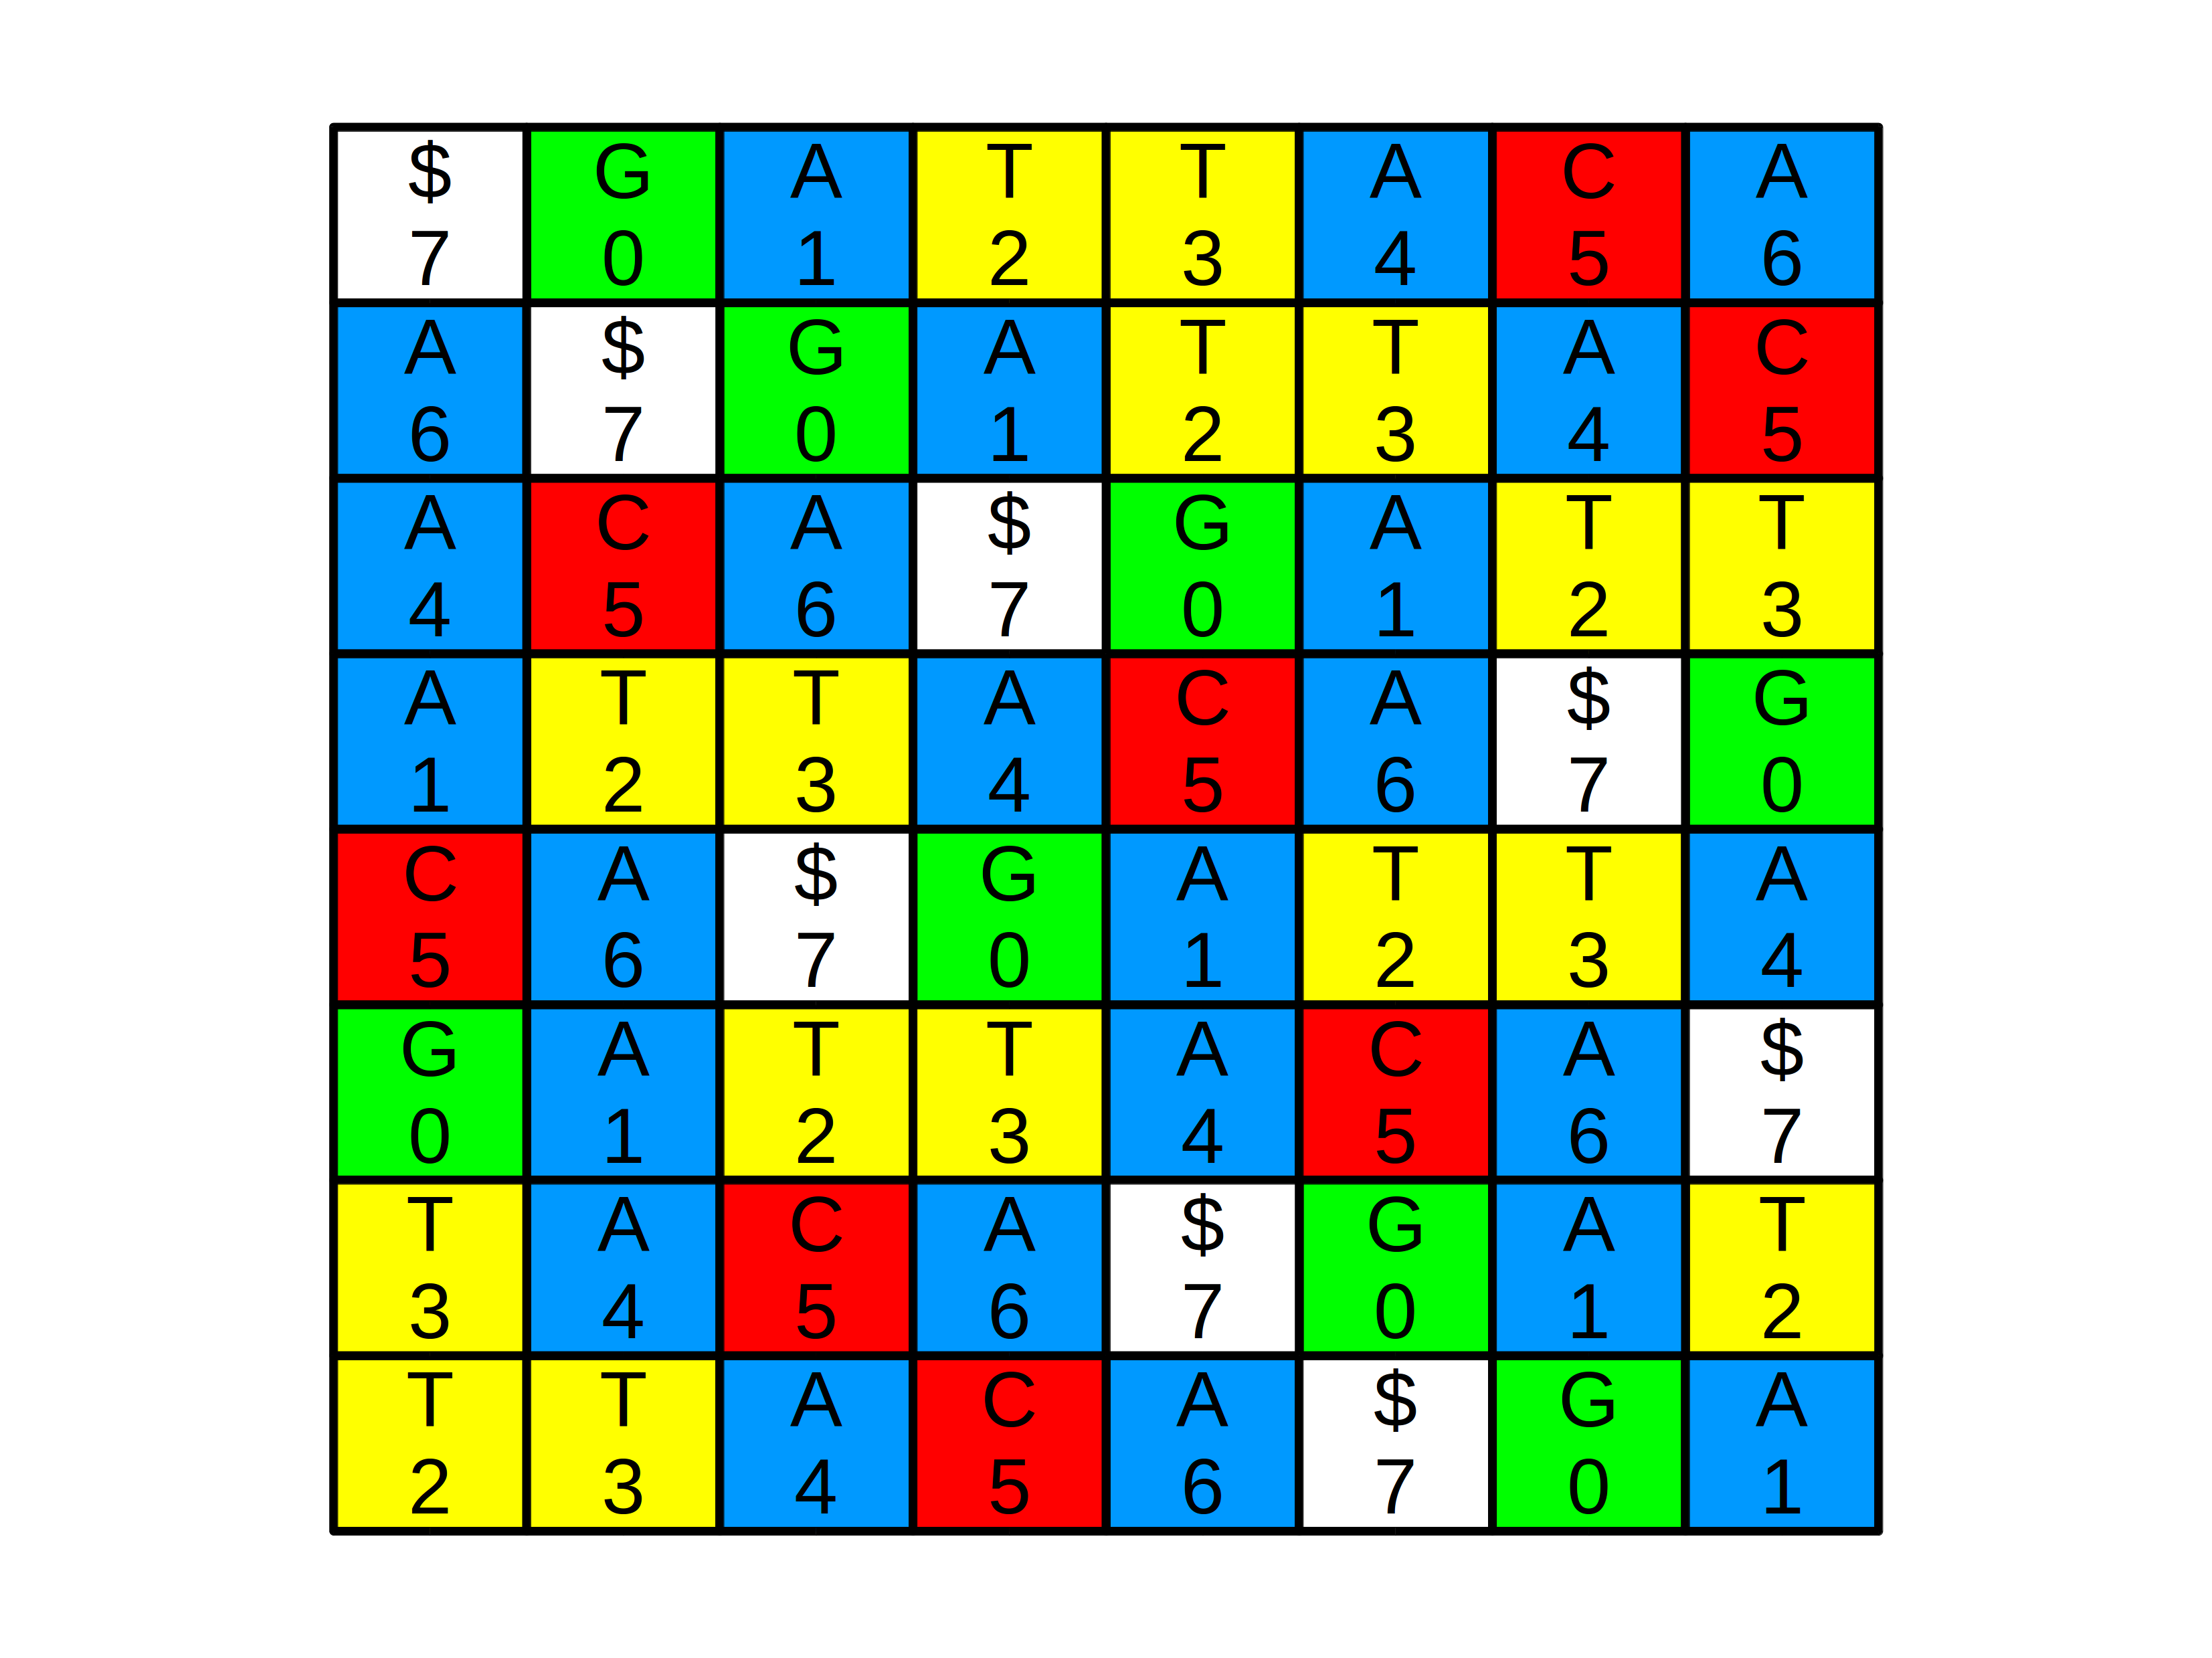
\includegraphics[width=1.0\textwidth]{figures/01_introduction/bwt.png}
    \caption[An example BWT matrix for the string ``GATTACA'']{An example BWT matrix for the string ``GATTACA''. The sentinel value ``\$'' is appended to the end of the string, all rotations of the string are calculated, and the rotations are sorted. Bases are colored according to base identity and numbered according to position in the original string. The characters in the far right column are the BWT of the original string, while the numbers in the far left column are the suffix array (represented as indices into the original string).}
    \label{fig:bwt}
\end{figure}

Note that the instances of any given character in the last column appear in the same relative order in the first column. Consider just the rows where the character in question appears in the first column. When sorting these rows, the first column is uninformative (since it is constant across all rows), and the rows are sorted lexicographically by the remaining columns in order. Rotating all the strings so the uninformative column appears last will not change the order of the other columns, and thus will not change the relative sort order of the rows we are considering. Thus the instances of the character stay in the same relative order in the last column as in the first column \cite{langmead2013introduction}.
    
\subsection{Substring Search with the Suffix Array}

The \vocab{suffix array} of a string is an array of indices into the string, sorted in the lexicographical order of the suffixes that they point to \cite{manber1993suffix}. For example, the string ``dog'' has suffixes ``dog'' at index 0, ``og'' at index 1, and ``g'' at index 2, so its suffix array would be $[0, 2, 1]$, corresponding to the suffix sort order $[\textrm{``dog''}, \textrm{``g''}, \textrm{``og''}]$. Another example suffix array is visible in the leftmost column of Figure~\ref{fig:bwt}.

Suffix arrays have some useful properties. Most importantly, all of the suffixes that start with the same substring appear in a single contiguous block \cite{ferragina2000opportunistic}. This block starts at the position corresponding to the number of occurrences of lexicographically smaller substrings of the same length \cite{ferragina2000opportunistic}. This is particularly obvious in the case of single-character substrings: all the suffixes (and, thus, all the substrings) beginning with a certain character appear in one block, coming immediately after all suffixes beginning with lexicographically smaller characters.

Suffix arrays can be used as indices to speed up substring search on the string they are derived from. Because of the block structure described above, and because every instance of a substring is at the beginning of some suffix, a simple binary search is sufficient to find any substring that is present, and a scanning up and down from one instance can pull out the entire corresponding block \cite{manber1993suffix}. Supplementing the suffix array with a \vocab{longest common prefix (LCP)} array, holding the length of the prefix shared by each pair of adjacent suffixes, can further speed up the search, by requiring only a single-character comparison (instead of a string comparison) at each search step \cite{manber1993suffix}.
    
\subsection{Searching in BWTs with the FM-index}

Constructing the BWT matrix is essentially the same task as constructing the suffix array of the string being transformed. All the rotations of the string contain the ``\$'' sentinel which is lexicographically less than all other characters. Thus the rotations are actually sorted by the portion before the ``\$'' character---that is, by the corresponding suffixes of the original string. This is the same sort used to construct the suffix array.

A BWT can be augmented with a small amount of additional information to create an FM-index (named after its inventors), which, like a suffix array, allows efficient substring search on the original string, but which also retains the compression afforded by the BWT \cite{ferragina2000opportunistic}. The FM-index is based primarily on the idea of an LF (i.e. last-first) mapping. This mapping maps each character instance in the last column of the BWT matrix to the row in which that same character instance appears in the first column. Because each BWT matrix row is a rotation of the original string, the last column of the row will contain the character instance immediately preceding the one just looked up. Thus, following the LF-mapping around the BWT from any starting position allows the characters of the original string to be enumerated from there in reverse order \cite{ferragina2000opportunistic}.

Since only the last column of the BWT matrix (i.e. the actual BWT string) is used in the algorithm, only that string needs to be stored. Furthermore, the LF-mapping can easily be calculated from the BWT string. To LF-map the character instance at a certain index in the BWT, count up the number of characters in the BWT lexicographically less than the character, and add the character instance's rank among all instances of that character. This gives the index of the LF-mapping result in the BWT.

To see why this works, recall that in a suffix array, and thus also in the BWT matrix, all the suffixes (or here rotations) that start with a given character form a contiguous block, coming just after all those beginning with smaller characters. Thus, the first calculation is to find the start of this block. And since, as shown in Subsection~\ref{subsec:bwt}, the relative order of character instances in the first column is the same as that in the last column, to find the offset of this particular character instance in that contiguous block, we merely need to find its rank among instances of the same character in the last column, which is the BWT string \cite{langmead2013introduction}.

We can now define \vocab{backward search}, a search algorithm using the BWT which processes the characters in the query string from back to front. The algorithm begins by selecting the entire BWT matrix, which is the range of suffixes that begin with the empty string. Then, for each character in the query string, from the last forwards, the algorithm extends the searched string at the front with that character. It takes the new character and finds the first and last instances of it in the BWT contained within the currently selected result range. It then LF-maps each of those instances, and takes the range between them as the new result range for the query string extended with that character. If there are no instances of the character to map, then the searched string is not found in the index \cite{ferragina2000opportunistic}.

Each row of the BWT matrix in the old range started with an instance of the old query string. Each of the rows that ended in the new query character corresponded to an instance of the old query string occurring after the new query character, and thus each implies an instance of the new, one-character-longer query string. The LF-mapping step finds the contiguous block of rows in the BWT matrix where those instances of the search string appear, the boundaries of which correspond to the first and last instances of the new character in the old BWT range (by the conservation of ordering mentioned at the end of Subsection~\ref{subsec:bwt}). Thus, such an algorithm can be used to search for substrings in a string, using the BWT of the string \cite{ferragina2000opportunistic}.

By pre-calculating some auxiliary data structures, such as a table with the start index of each character's range in the BWT matrix, and by using succinct data structures for $O(1)$ rank queries, this algorithm can be made to run in time linear in the length of the query string, and constant in the length of the index \cite{ferragina2000opportunistic}. Furthermore, using a downsampled copy of the suffix array, the location of each result in its source string can be calculated efficiently \cite{siren2009run}.

\subsection{Bidirectional DNA Search with the FMD-Index}

BWT-based indices have found many applications in genomics, mostly due to their ability to efficiently search for and identify the locations of a substrings in very large data sets---with a few modifications, this search can be extended to align reads to a reference \cite{li2014bwa}. The popular short read aligner \texttt{bwa}, for example, is built on an FM-index of the reference genome; indeed, the name stands for ``Burrows--Wheeler Aligner'' \cite{li2014bwa,li2009fast}. The ``String Graph Assembler'' \texttt{sga} also uses a BWT-based index to do its work, but in this case indexes reads themselves \cite{simpson2012efficient}.

In genomics, the strings being indexed are DNA strings, consisting of As, Gs, Cs, and Ts. These DNA strings are usually excerpts from double-stranded DNA genomes, in which, for each chromosome, two strands of DNA form a double helix. One strand runs in one direction, and the other strand runs in the other direction, with bases complemented (As and Ts swapped, and Gs and Cs swapped). It's impossible to tell whether a DNA sequencing read came from the forward strand or the reverse-complement strand until a match is found for it in a reference somewhere. Thus, many analysis problems in genomics need to consider not only some set of DNA strings but also their reverse complements.

The existence of reverse complements is accounted for in \texttt{sga} by creating two FM-indices of the input data: one index of the forward strand, and one of the reverse-complement strand \cite{simpson2012efficient}. This construction requires DNA query strings to be searched against both indices, and the results combined. However, there is a more elegant approach which allows the same search to be performed against a single index, and moreover allows bidirectional extension of the query string. This data structure, the ``FMD-index'' (the ``D'' is for ``DNA''), is simply an FM-index of both the forward and reverse strands of all input sequences, concatenated into a single data set \cite{li2012exploring}.

The FMD-index provides for double-ended search; that is, an intermediate search result can be extended with a character on either the left or right end of the query string. This works by having the FMD-index store as its intermediate result not just the single range in the BWT corresponding to BWT matrix rows that start with the query string, but also the (equally long) range for the reverse complement of the query string \cite{li2012exploring}. The first is the \vocab{forward range} and the second the \vocab{reverse range}. The fact that these two intervals will always be equally long is the key to the algorithm: because each string in the index is present as both itself and its reverse complement, any appearance of the query string has a corresponding appearance of its reverse complement. Extending the query string on the left causes the forward range to jump around in BWT coordinate space (to the regions of the BWT matrix that begin with the newly added character). However, extending on the left always causes the reverse range to cover a subrange of what it covered previously: the reverse complement of the query string gets extended on the right, and only BWT matrix rows which began with the original reverse-complement query string can possibly also begin with the longer reverse-complement query string.

The FMD-index search algorithm works as follows: When the query string is extended on the left, the forward range is updated as normal. The reverse range takes on the new interval length derived from the forward range, and a small dynamic programming problem is done over the alphabet to find its new start position. The dynamic programming problem is fairly simple because the reverse range can be partitioned into the ranges that would be selected upon left-extension with any character, ordered in lexicographic order by the reverse complement of the character. The dynamic programming simply consists of looping through the alphabet in lexicographic order by reverse complement, considering extending on each character up to the one actually being used, calculating how long the result set would be on the forward strand, and adding that in to the start of the reverse strand interval \cite{li2012exploring}. To extend a string on the right, the forward and reverse ranges are temporarily swapped, and the reverse complement of the query string is extended on its left with the reverse complement of the new base \cite{li2012exploring}.

% TODO: what if this BWT stuff can I cut, given that I'm no longer trying to use my own FMD index implementation to represent a merged-from-sequences graph?

\subsection{Previous Graph Indices}

% Improve this paragraph to actually say what is actually happening
A graph-based Human Genome Variation Map requires an efficient substring search algorithm, in order to allow sequencing reads to be efficiently aligned to the graph. Substring search in graphs is not a new idea. Many of the current approaches to this problem come at it from the perspective of trying to index a multiple sequence alignment \cite{siren2014indexing}. Two such approaches are described below.

One approach, the Generalized Compressed Suffix Array (GCSA), extends the XBW transform (itself a generalization of the BWT to trees) to ``prefix-range-sorted automata'', which include de Bruijn graphs but not general directed labeled graphs \cite{siren2014indexing}. However, the authors of that approach present only an implementation for acyclic multiple sequence alignments. The existence of nonlinear structures like polymorphic inversions, where a genomic region is forwards in some individuals but backwards in others, is not addressed, and no implementation for de Bruijn graphs is provided \cite{siren2014indexing}. Moreover, the approach presented there provides search over all possible paths through the graph in question, which is a reasonable choice for indices derived from multiple alignments, but which might backfire for graphs with short cyclic structures that could provide pathological productions for many query strings \cite{siren2014indexing}.

Another, slightly newer approach uses the concept of a ``population reference graph'', also derived from a multiple sequence alignment \cite{dilthey2015improved}. In contrast to the BWT-based indexing methods described above, the population reference graph method turns its graph representation of genomes into a Hidden Markov Model (HMM), and identifies the most likely paths through it to match the k-mer spectrum of any particular sample \cite{dilthey2015improved}. Under this method, a pair of haploid genomes are then synthesized as sample-specific references, and existing read-to-genome mapping tools are used to map sequencing reads to these references \cite{dilthey2015improved}. Unfortunately, because of the way that k-mer counts from a sample are divided up to provide input for the HMM model in different genomic regions, this method is forced to divide its HMM states into ``levels'' that it proceeds through in a fixed, sequential order. The resulting graph model is constrained to closely resemble the multiple sequence alignment it was derived from. While this method can effectively model a wide range of alternative sequences in a region, it does not appear to be able to effectively model inversions, duplications, or other more complex structures \cite{dilthey2015improved}.

% TODO: Talk about and cite GCSA2 which actually gets used

% Maybe hit the vBWT as well

\subsection{Sequence Graphs}

There are many possible representations of a genomic reference as a graph \cite{computational2016computational}, but one particularly useful model is a bidirected graph, or, when used to represent genomic data, a \vocab{sequence graph} \cite{paten2017genome}. In the sequence graph model, nodes in the graph are nucleic acid \vocab{sequences}, and each sequence has two \vocab{sides}: a ``left'' or ``start'' side and a ``right'' or ``end'' side. The sequences are connected together by \vocab{edges}, each of which has two ends that are attached to sides of nodes. The model is called ``bidirected'' because, unlike in a directed graph where each edge consists of a set of nodes and a direction (from one node to another), in a bidirected graph each edge consists of a set of nodes and two directions. The edge can still be from one node to another (in which case it connects the end side of one node to the start side of the other), but it can also be ``to`` both nodes (in which case it connects their start sides together), or ``from'' both nodes (in which case it connects their end sides together).

In a graph such as this, traversals, walks, and other graph-theoretic concepts generalize from visiting just the nodes to visiting nodes in one of two orientations: \vocab{forward} (i.e. start side to end side) or \vocab{reverse} (i.e. end side to start side). A visit to a node in the forward orientation corresponsd to the node's sequence, whereas a visit to the node in the reverse orientation corresponds to the reverse complement of its sequence. When visiting multiple nodes, it is important that the visits' orientations be consistent: if two nodes are connected by an edge from the first to the second, and you visit the first node in its forward orientation, you may next visit the second node in its forward orientation (by leaving the first node's end and arriving at the second node's start), but you may not, traversing that edge, visit the second node in its reverse orientation. In other words, the forward orientation corresponds to arriving at the start side and leaving via the end side, whereas the reverse orientation corresponds to arriving at the end side and leaving via the start side, and other combinations (such as both arriving and leaving via the start side) are not permitted.

% TODO: a figure might be nice here.

\subsection{Data Models with Protobuf}

Representing human genomic variation as a graph reference requires a data model in which to represent that graph in software. Moreover, producing an effective Human Genome Variation Map that can actually be used by other researchers requires selecting a data model that can itself be easily communicated, that can have broad software support, and that people can be persuaded to agree on.

A simple way to describe a data model and get code generated in various languages for free is to use Google's Protocol Buffers (or ``Protobuf'') library \cite{varda2008protocol}. The system provides a simple language to describe data structures, and a serialization system to allow multiple languages to read and write those data structures. The availability of libraries such as \texttt{json2pb} allows easy interoperation with any languages or tools that can consume or produce JSON. Additionally, the relative sparsity of features forces data models to be relatively simple, and the backing by a large, rich technology company helps convince people to agree on the format. Finally, the extensibility of the system allows new fields to be added to provide new features without invalidating older data sets.

Here is an example Protobuf description of a graph node in a genome graph. 

\begin{lstlisting}
// *Nodes* store sequence data.
message Node {
    string sequence = 1;   // Sequence of DNA bases represented by the Node.
    string name = 2;  // A name provides an identifier.
    int64 id = 3;     // Each Node has a unique positive nonzero ID within its Graph.
}
\end{lstlisting}
% TODO: Word wrap this

Each kind of item in the data model is referred to as a ``message'', and each field is manually assigned a unique identifying number to allow its name to be changed later while retaining backward compatibility.

Using a Protobuf-based data format for genome graphs allows for broad accessibility, without some of the disadvantages (such as large size and the necessity to write correct parsers in various languages) of bespoke text formats.

\subsection{\vg, the Variation Graph Toolkit}

% I should talk about vg, at least as it existed before I started working on it.

One collection of Probuf data models for genome graphs comes from \vg, a software suite created by Erik Garrison for working with genome graphs \cite{garrison2016vg}. In \vg, graphs are represented by a collection of nodes, each of which has an ID and a sequence, and a collection of edges, each of which connects one side (the start or end) of one node to one side of another node (which may actually be the same node, because the \vg model allows for cycles and self-loops). Each graph can also have a series of named paths associated with it, to represent how interesting things, such as the primary path of a genome assembly, or the reference version of a particular gene, fit into the graph.

The \vg suite is structured as a command-line \vg command with a variety of subcommands (\texttt{vg construct}, \texttt{vg map}, \texttt{vg view}, etc.), which are designed to be chainable into pipelines and communicate using streams of Protobuf-serialized graph data. The toolkit, The combination of the Protobuf-based serialization format, the modular architecture as a collection of subcommands, and the relatively comprehensive internal graph manipulation API make \vg and attractive option as a framework in which new genome graph algorithms can be implemented, and a useful toolkit for performing graph-based analyses.

At the time when \vg was selected as a basis for further development, it provided a data model supporting bidirected graphs, subcommand implementations for constructing, indexing, and mapping to directed acyclic graphs, and a succinct graph storage format. In part as a result of software development work undertaken as part of the present work, \vg now includes full support for working with bidirected graphs, a variant calling implementation, and a suite of unit tests.

\subsection{Copy-Number-Variable Alignments with Cactus}

When building a Human Genome Variation Map, it would be desirable to be able to incorporate variation data in the form of observed sequences, such as the European-representative MHC sequences obtained in \citet{horton2008variation}, or the many alt loci sequences provided with GRCh38 \cite{karolchik2014new}. Thus, it is necessary to have a mechanism to go from a collection of related sequences to a graph representation describing their commonalities. The \vg suite includes a tool designed to do this, \texttt{vg msga} (which stands for ``multiple sequence graph alignment''), but this tool remains under active development.

An alternative approach is to use a more mature multiple aligner tool called Cactus \cite{paten2011cactus2}. The Cactus aligner, which has been deployed in production for the production of community alignment resources \cite{howe2015wormbase}, was designed for alignment problems involving large numbers of whole genomes, and consequently understands the sorts of structural changes between genomes, such as large-scale deletions, duplications, and rearrangements, that need to be dealt with when working at those evolutionary time scales. Cactus output typically takes the form of a Hierarchical Alignment Format (HAL) file \cite{hickey2013hal,howe2015wormbase}, which uses a phylogenetic tree with internal ancestor nodes to structure information about how blocks of different genomes relate to each other. The structure formed by relationships between corresponding blocks in different genomes is quite similar to a sequence graph, with the genomes being embedded in it as paths, and so Cactus-based alignments have a natural conversion to sequence graphs.

\subsection{Reliable, Portable Cloud Computing with Toil}

% Talk about how great Toil is and how it let me do lots of the analyses in here

In order to produce a graph reference on the scale of the proposed Human Genome Variation Map, using tools like \vg that are architected as small components performing relatively simple tasks, some sort of orchestration or workflow system is necessary. This is especially true if one desires to use more than one computer in the build process; tasks need to be scheduled and code and data moved around the cluster of systems in order to perform the build. Moreover, a build process like this might require more computing resources than are required to work with the final product, and so it is desirable to be able to source those resources from on-demand cloud providers, rather than being forced to purchase them in-house.

One potential solution to this problem is Toil, a Python-based workflow development library and execution engine which is capable of composing smaller tasks into larger workflows, and of executing those workflows either on a single computer or on a cloud-based virtual cluster \cite{vivian2017toil}. Toil workflows can be written as Python scripts, which, together with Python virtual environments housing their dependencies, can be distributed to worker machines in a cloud environment. Toil nodes comunicate amongst themselves using a \vocab{job store}, which can be located on a shared filesystem or within a cloud-based distributed storage system such as Amazon's S3 or Microsoft's Azure Storage. The job store is used to keep track of which parts of the workflow have successfuly completed, and which parts have not yet executed or have failed, as well as to store files, arguments, and return values that are communicated from job to job.

Toil jobs can dynamically create and connect additional jobs in a directed acyclic dependency graph, meaning that workflows can dynamically adapt their shape to the shape of the data they are working with. Moreover, because the information required to execute each job is stored in the job store, failed jobs can be retried, and jobs suffering from bugs can be restarted with a corrected version of the workflow code, allowing problems with a large workflow to be corrected without losing all of the work done so far.

To make running on cloud providers easier, Toil provides a system to control workflow input and output, by importing data from URLs at the beginnig nof the workflow, and exporting data to URLs at the end, to eliminate the need to manually copy data to and from ephemeral cloud instances. Additionally, Toil provides a Python API for running commands through the Docker container system, allowing workflows to call command-line tools without the user having to figure out a way to get them installed on large numbers of ephemeral cloud instances. Finally, Toil integrates with Amazon Web Services to allow clusters to be automatically scaled up and down as the resource requirements of a workflow change, or as the spot market price of computing-hours rises and falls, while for Microsoft Azure Toil provides a cluster template for easy deployment in a few clicks.

\section{Research Overview}

% Maybe this is where I should talk about tying together all the cools tuff I did and why I made the decisions I made



% Chapter 2 describes the formal mapping mathematics work that I did, and is
% derived from the "Canonical, Stable, General Mapping Using Context Schemes"
% paper.
% Make floats less spacey. See <http://tex.stackexchange.com/a/26522>
\setlength{\textfloatsep}{1pt plus 1.0pt}

% Apparently we have to invent our own kinds of theorems
\newtheorem{theorem}{Theorem}
\newtheorem{lemma}{Lemma}

\chapter{Canonical, Stable, General Mapping Using Context Schemes}

\section{Abstract}
\subsection{Motivation:}
Sequence mapping is the cornerstone of modern genomics. However, most existing sequence mapping algorithms are insufficiently general.

\subsection{Results:}
We introduce context schemes: a method that allows the unambiguous recognition of a reference base in a query sequence by testing the query for substrings from an algorithmically defined set. Context schemes only map when there is a unique best mapping, and define this criterion uniformly for all reference bases. Mappings under context schemes can also be made stable, so that extension of the query string (e.g. by increasing read length) will not alter the mapping of previously mapped positions. Context schemes are general in several senses. They natively support the detection of arbitrary complex, novel rearrangements relative to the reference. They can scale over orders of magnitude in query sequence length. Finally, they are trivially extensible to more complex reference structures, such as graphs, that incorporate additional variation.
We demonstrate empirically the existence of high performance context schemes, and present efficient context scheme mapping algorithms.

\subsection{Availability and Implementation:}
The software test framework created for this work is available from \url{https://registry.hub.docker.com/u/adamnovak/sequence-graphs/}.

\subsection{Contact:} \href{benedict@soe.ucsc.edu}{benedict@soe.ucsc.edu}
\subsection{Supplementary Information:} Six supplementary figures and one supplementary section are available with the online version of this article.

\section{Introduction}

%%Benedict's proposed introduction - the reference numbers are all wrong.

Many tools and algorithms exist for mapping reads to a reference genome \citep{li2010fast,langmead2009ultrafast,harris2007improved}. These tools are based on the idea of scoring local alignments between a query string and a reference according to some set of match, mismatch, and gap scoring parameters, and then finding local alignments with maximal or near-maximal scores. Seed-and-extend approaches coupled with memory efficient substring indexes or hashing schemes have been highly successful in heuristically accelerating this search process \citep{dobin2013star,li2010fast,langmead2009ultrafast}. 

The core problem with read mapping is ambiguity. There is often no single best place that a read maps, especially in the case of recent duplication within the reference genome. The precise base-level alignment of the read to a given location in the reference is also often ambiguous. To mitigate this, each mapped read is given a mapping quality, a per read score that indicates how likely the mapping was generated erroneously \citep{li2008mapping}. Quantifying this uncertainty is a reasonable approach for many applications, but even then the uncertainty can be difficult to accommodate downstream.

The difficulty of mapping a read to a reference motivates a consideration of its necessity. Recently, alignment-free methods of variant calling through substring detection have garnered significant interest \citep{dilthey2014improved}. The basic idea is not new; the dbSNP database has long provided, for each point variant in the database, a flanking nucleotide string that indicates the DNA context in which the variation was isolated \citep{sherry2001dbsnp}. In principle such a system of variant identification sidesteps the limitations of score based alignment, and can be used to canonically detect variations. However, in practice, insufficient rigor in defining the substrings to detect, and a failure to account for other variation near identified point mutations have limited the approach's usefulness. Here we formalize and extend this core idea; we propose using multiple, algorithmically defined context strings to canonically identify the presence of each base within a reference genome (potentially paving the way for high-specificity, alignment-free variant calling) and evaluate the performance of such a method in practice. 

%Cut for brevity
%In its simplest form, each reference base is labeled by a ``context string'' that, when detected in a query sample, is sufficient to unambiguously identify the base’s presence. To account for the randomly placed boundaries of short sequencing reads, which would often inconveniently truncate any single context string for a reference base at one end or the other, and to accommodate other nearby variation, we generalize the notion from a single context string per base to a set of such strings per base. When such a system is applied across a reference genome it defines a mapping scheme; we call this a ``context-driven'' mapping scheme. We first define context-driven mapping schemes in general, then give a specific, useful scheme and develop associated algorithms for its implementation. Finally we demonstrate empirically its practicality for the mapping of assembled sequences, as well as individual reads.

%%End of benedict intro


% We want to do variant calling

% People tried to do variant calling without mapping.

% It turns out that that's hard

% So we present a new mapping method inspired by these attempts at reference-free variant calling


%Everybody in genomics wants to call variants. We already have an idea of what human genomes look like in general; when an individual is sequenced, the primary concern is how that individual differs from the human reference genome. This is usually determined by aligning sequencing reads from the individual against the reference genome, and explaining differences between the reads and the reference by invoking variants in the individual. However, read mapping is a complex and slow process; it only works as well as it does because of the thousands of hours of work people have spent on heuristic acceleration and optimization \citep{dobin2013star,li2010fast,langmead2009ultrafast}.

%The difficulty of mapping a read to a reference motivates a critical consideration of its necessity. Some approaches to variant calling rely instead on the identification of substrings within collections of reads in order to ascertain the presence or absence of genomic variants \citep{dilthey2014improved}%REF-DURBIN? POSSIBLY
% Citing Gil's HMM preprint thing
%. The dbSNP database caters to this view by attaching to each point variant in the database upstream and downstream flanking nucleotide strings that indicate the DNA context in which the variation was isolated \citep{sherry2001dbsnp}. In principle, this would allow dbSNP variants to be identified in a reference-free way. However, insufficient rigor in defining appropriate context strings, and a failure to account for other variation near the identified point mutation has limited the use of these sequences in practice.  

%%Overview of method, which combines notion of context sequences

%What is needed is a middle ground between traditional read to reference genome alignment and reference-free methods of variant detection. We would like to preserve the idea of a space in which variants exist, while phrasing uses of read data in terms of simple and formally tractable substring operations. 

%Here we propose using context strings to canonically identify the presence of each base within a reference genome. We build on the idea of labeling each reference base with a ``context string'' that, when detected in a query sample, is sufficient to unambiguously identify the base's presence. To account for the randomly placed boundaries of short sequencing reads, which would often inconveniently truncate any single context string for a reference base at one end or the other, and to accommodate other nearby variation, we generalize the notion from a single context string per base to a set of such strings per base. When such a system is applied across a reference genome it defines a mapping scheme; we call this a ``context-driven'' mapping scheme.

%We first define context-driven mapping schemes in general, then give a specific, useful scheme and develop associated algorithms for its implementation. Finally, we empirically demonstrate our method's practicality for the mapping of assembled sequences, as well as individual reads.


\section{Methods}

%Define genome, reference genome and input sequence

%Definition of a mapping function

%%Mention how we deal with multi-mapping (point at hierarchy stuff in other paper).

%Definition of a context scheme

%Properties of a context scheme
%%Stability
%%Non-linearity
%%Extension to graphs
%%Uniqueness/functional mapping

Throughout we make use of \vocab{DNA strings}, which are finite strings over the alphabet of \vocab{DNA bases} $\left\{\mathrm{A}, \mathrm{C}, \mathrm{G}, \mathrm{T}\right\}$. 
%Removing for brevity. This is unnecessary in my opinion.
%A DNA string $x$ has \vocab{elements} $1$ through $n$; each element $i$ in $x$ has a \vocab{base} $x_i$ that appears in the string at index $i$. 
A DNA string $x$ has a \vocab{reverse complement} $x^*$, which is the reverse of $x$ with each DNA base replaced with its complement; $\mathrm{A}$ and $\mathrm{T}$ are complements of each other, as are $\mathrm{G}$ and $\mathrm{C}$. 

\subsection{Mapping}
A \vocab{reference (genome)} $G$ is a set of DNA strings and an index set of the elements of these strings, each member of which is called a \vocab{position}. Each position $p$ uniquely identifies an element $b(p)$ of a string in $G$. This allows us to unambiguously discuss the ``positions'' in that set of DNA strings, rather than ``bases'' or ``characters'', which could be interpreted as the four DNA bases themselves.

 We define the problem of mapping a \vocab{query} DNA string $x=(x_i)_{i=1}^n$ to a reference $G$. 
A \vocab{mapping scheme} is a function that takes $x$ and $G$ and, for each query element $i$ of $x$, either returns a position in $G$, declaring the query element $i$ to be \vocab{mapped} to that position in $G$, or declares the query element to be \vocab{unmapped} in $G$. For the scheme to map a query element to a position $p$ in $G$, $b(p)$ must either be $x_i$ (in which case that query element is \vocab{forward mapped}), or ${x_i}^*$ (in which case that query element is \vocab{reverse mapped}). 

\subsection{Contexts}
A \vocab{context} is a tuple $(L, B, R)$, where $L$ is a DNA string called the \vocab{left part}, $B$ the base, and $R$ is a DNA string called the \vocab{right part}. The string $LBR$ is the \vocab{context string} of the context $(L, B, R)$. The context distinguishes $B$ from the rest of the context string, so that when the context is found to occur in a query string, it is clear which character in the query string (i.e. the one corresponding to $B$) has been recognized.
For an element $i$ in a DNA string $x$ a context $(L, B, R)$ is called a \vocab{natural context} if $B=x_i$,  $L$ is a (possibly empty) suffix of $(x_j)_{j=1}^{i-1}$ and $R$ is a (possibly empty) prefix of $(x_j)_{j=i+1}^n$. Some example natural contexts are visible in Supplementary Figure~S1. % We need this since we are going to want to assign contexts with mismatches later that don't actually appear in the strings in the reference


\subsubsection{Context Generality}
A context $c_1 = (L_1, B_1, R_1)$ is \vocab{forward more general} than a context $c_2 = (L_2, B_2, R_2)$ if $L_1$ is a suffix of $L_2$, $B_1 = B_2$, and $R_1$ is a prefix of $R_2$. That is, if you turned the two contexts into strings with their bases marked as special characters, the more general context would be a substring of the \vocab{less general} context. Note that a context is forward more general than itself. A context $c_1$ is \vocab{reverse more general} than a context $c_2$ if $c_1$ is forward more general than the reverse complement of $c_2$, which is $c_2^* = (R_2^*, B_2^*, L_2^*)$. We define a context $c_1$ to be generically \vocab{more general} than context $c_2$ if it is either forward more general or reverse more general than $c_2$. 
%Cut for brevity
%We use the term \vocab{(forward/reverse) less general} for the inverse relation.

\subsection{Context-Driven Mapping}
It is possible to define a mapping scheme for a query string $x$ to a reference $G$ in terms of contexts for positions in the reference. Such a mapping scheme makes use of a context assignment.

\subsubsection{Context Assignment}
A \vocab{context assignment} assigns each position in a reference a nonempty \vocab{context set}, such that all contexts in the set have the same base as the position, and no context in one position's set is more general than any context in any other position's set (Figure \ref{fig:contextSets}). This second property of context assignments is called \vocab{nonredundancy}.  
%Cut for brevity
%Note, however, that it is possible for two contexts from different context sets, neither of which is more general than the other, to both be more general than some context in which a query base is observed; nonredundancy does not guarantee nonambiguity.

\subsubsection{Matching}
An element $i$ in a query string $x$ is said to \vocab{match} a context $c = (L, B, R)$ if the query, when partitioned into the context $((x_j)_{j=1}^{i-1}, x_i, (x_j)_{j=i+1}^n)$, is less general than $c$. Note that this encompasses both forward less general (in which case element $i$ \vocab{forward matches} the context) and reverse less general (in which case element $i$ \vocab{reverse matches} the context). When the context is in the context set of a reference position, the element \vocab{matches} the position \vocab{on} the context. 

%Cut for brevity
%Elements can also match positions. An element $i$ in a query DNA string is said to \vocab{match} a position $p$ in a reference under a context assignment $C$ if element $i$ matches some context in $p$'s context set assigned by $C$. If $i$ forward matches the context this is \vocab{forward matching}, and if $i$ reverse matches the context this is \vocab{reverse matching}. (Note that due to the requirements on the base of a context it is impossible to both forward match and reverse match the same position.) Element $i$ is said to \vocab{match on} the context.

\subsubsection{Context-Driven Mapping Schemes}
% This paragraph starts on the same line as the subsubsection title and wants to escape the margins.
\begin{sloppypar}
A \vocab{context-driven mapping scheme} is a mapping scheme which, for query $x$ and reference $G$ with context assignment $C$, maps each element $i$ in $x$ to the unique position in $G$ which it matches under $C$, or leaves $i$ unmapped when no such position exists. An element remains unmapped when it does not match any context of a reference position, or when it matches contexts of two or more positions; in the latter case we say it \vocab{discordantly matches}, an example of which is visible in Supplementary Figure~S2.
\end{sloppypar}


Under a (nonredundant) context assignment, each position $p$ in the reference can be mapped to, because for each context $(L, B, R)$ of $p$ the context string $LBR$ matches $p$ on that context. The nonredundancy requirement ensures this matching is not discordant: no context more general than $(L, B, R)$ can be in the context set of any other position in the reference.

\subsubsection{Stability}
An \vocab{extension} of a DNA string $x$ is a DNA string that contains $x$ as a substring.  
An element $k$ in an extension $x'$ of $x$ is a \vocab{partner} of an element $i$ in $x$  if the context $((x_j)_{j=1}^{i-1}, x_i, (x_j)_{j=i+1}^n)$ is more general than $((x'_j)_{j=1}^{k-1}, x'_k, (x'_j)_{j=k+1})$.

A mapping scheme is \vocab{weakly stable} 
if for each element $i$ in each possible query string $x$, if $i$ is mapped to a position $p$ in the reference, its partners in all extensions of $x$ will map to $p$ or be unmapped.
Weak stability is desirable because it guarantees that an element in a query cannot change its mapping to a different position under extension---the mapping scheme never has to admit that it mistook one reference position for another when presented with more information. Unlike score based mapping procedures, which are generally not weakly stable, all context-driven mapping schemes are weakly stable, because for any mapped element $i$, the partners of $i$ in an extension of the query string can only either map to the same position $p$, or be discordantly matched and therefore unmapped. This is because these partners have all the natural contexts of $i$, and therefore must match on a context in the context set of $p$, but may additionally match on the context of a different position in the reference and therefore discordantly match.
%\subsubsection{Stable Context-Drive Mapping Schemes}

A mapping scheme is \vocab{stable} 
if for each element $i$ in each possible query string $x$, if $i$ is mapped to a position $p$ in the reference, its partners in all extensions of $x$ will map to $p$. Stability is naturally a more desirable property than weak stability, as it restricts mapping to individual positions aligned with high certainty.
%, because once mapped an element in a query string remains mapped to the same position under extension.
By the argument above, some context-driven mapping schemes are only weakly stable. A \vocab{stable context-driven mapping scheme} is equivalent to a context-driven mapping scheme that additionally makes an element of a query string unmapped if a partner element in any extension of the query would discordantly match. 
%This is unnecessary.
%Although it might seem obvious, it is important to note that a ``stable context-driven mapping scheme'' is stable as defined above.

\begin{figure}
  \begin{minipage}{0.5\linewidth}
  \centering
  \begin{tabular}{rcl}
  \multicolumn{3}{c}{Contexts for position $P_1$} \\ \hline
  $(L,$ & $b,$ & $R)$ \\ 
  \texttt{TGTCGC} & \texttt{C} & \texttt{CAAGCA} \\ 
  \texttt{TG\textbf{G}CGC} & \texttt{C} & \texttt{CAAGCA} \\ 
  \texttt{TGTCGC} & \texttt{C} & \texttt{CA\textbf{C}A} \\ 
  \end{tabular}
  \end{minipage}%
  \begin{minipage}{0.5\linewidth}
  \centering
  \begin{tabular}{rcl}
  \multicolumn{3}{c}{Contexts for position $P_2$} \\ \hline
  $(L,$ & $b,$ & $R)$ \\ 
  \texttt{ACGAC} & \texttt{C} & \texttt{CCAG} \\ 
  \texttt{CGAC} & \texttt{C} & \texttt{C\textbf{T}} \\ 
  \texttt{ACGAC} & \texttt{C} & \texttt{CCA\textbf{T}G} \\
  \end{tabular}
  \end{minipage}

  \caption{Example of two nonredundant context sets. Substitutions relative to the first context in each set are in bold. If the context $(L, B, R) = \texttt{C}, \texttt{C}, \texttt{C}$ were added to either set, it would make the context assignment redundant, as it is more general than contexts that already occur in both sets.}
  \label{fig:contextSets}
\end{figure}

\subsection{The Natural Context-Driven Mapping Scheme}

%%Point to earlier paper for previous schemes.
In our earlier paper \citep{paten2014mapping} we discussed a number of different context assignments, including fixed $k$-mer approaches. Here we focus on a new scheme that is easy to reason about and which performed the best in our preliminary empirical tests (Supplementary Figure~S3).

%The Natural mapping schemes

The \vocab{natural context assignment} assigns to each position in the reference the subset of its natural contexts that are not natural contexts of any other position in the reference. It is trivially nonredundant.
%Need a figure to illustrate this
% Do we really?
The \vocab{natural (context-driven mapping) scheme}, which uses the natural context assignment, has an intuitive interpretation: an element $i$ of a query string is mapped to a position $p$ of the reference when all natural contexts of $i$ with context strings unique in the reference are are assigned to $p$.

%Algorithms for natural context schemes
%%%Define max unique substrings and inchworm recursion, keep it very brief.
\subsubsection{Overview of Algorithms}
The natural context scheme is also simple to implement. For a reference and query, a \vocab{maximum unique match (MUM)} is a maximum length substring of the query present once in the reference. % TODO: Does this adequately exclude the idea that we can take a MUM that has a longer version somewhere else in the query and declare it not a MUM?
Our definition of a MUM differs from that used by tools like MUMmer \citep{delcher1999alignment} in that it is nonsymmetric; we allow a MUM to have multiple \vocab{MUM instances} in the query, each of which is a MUM and an interval of the query corresponding to a location of the substring. For a query $x$ of length $n$ there are at most $n$ MUM instances, since two cannot start at the same place. Each MUM instance that contains a given element $i$ can be described as a natural context string of $i$: $(x_j)^{i-1}x_i(x_j)_{i+1}$. Under the natural context assignment, the context of each such MUM-derived context string matches exactly one reference position. %Each element $i$ in $x$ can be contained in no more (and probably far fewer) than $n$ MUM instances. 


Using a suffix tree with suffix links of the strings in a reference (which can be constructed in time linear in the sum of the length of the reference strings), or a related substring index data structure, it is possible to find the set of MUM instances for a query string ordered by ascending start element in $O(n)$ time. These data structures all provide two $O(1)$ operations, \vocab{extend} and \vocab{retract}, which, given a search result set for some search string, can produce the result set for a search string one character longer or shorter, respectively. Employing these operations to find all MUMs in order by ascending query start position is straightforward. Starting with the empty string, extend the search string on its right end with successive characters from the query string until such an extension would produce a search result set with no results (or until the query string is depleted). If at that point there is one result in the result set, and at least one extension has happened since the last retraction, then a MUM has been found. Next, retract a single character from the left end of the search string, and go back to extending with the remaining unused query string characters. Repeat the whole process until the query string is depleted.


%Cut for brevity (is redundant to above) When no more extends can be performed without losing the single unique result, the query substring represented by the search string is unique and maximal on the right. If, additionally, at least one extend has happened since the last retract, then this match is also maximal on the left. (If it was not, the most recent extend would have been performed before the most recent retract.)  

Since each successful extend operation consumes a character from the query string, no more than $O(n)$ extend operations can ever be performed. Since each retract operation moves the left end of the search string to the right in the query, no more than $O(n)$ retract operations can be performed. And since each unsuccessful extend operation (which would produce an empty result set) is followed by a retract operation, no more than $O(n)$ of those can happen either. Thus the entire algorithm is $O(n)$. 

Once the MUM instances have been found, it is necessary to identify the query elements that occur in exactly one MUM and therefore can be mapped under the natural scheme. (If an element is contained in two or more MUM instances then it must be discordantly mapped, because each must define a context that matches the element to a distinct position.) Given the MUM instances ordered by ascending query start element, it can be determined for all elements if each is in one, zero or multiple MUM instances, by a single traversal of the ordered MUM instances taking $O(n)$ time. We can therefore determine in $O(n)$ which elements in a query string are mapped. The combined time to map all the elements in a new query string given an existing reference substring index data structure of the type discussed is therefore $O(n)$.

\subsection{The $\alpha$-$\beta$-Natural Context-Driven Mapping Scheme}

%Introduce \alpha hamming separation of context strings
Under the natural context assignment, for each (by definition minimally unique) reference context string, there must exist another reference substring that is an edit distance of one from it.  Therefore, while the natural context assignment ensures each context identifies a single position in the reference, a single substitution, insertion or deletion in a query substring could result in a change in mapping. To avoid this, we now define a more robust scheme.

Throughout, we use the Levenshtein edit distance, in which a single character replacement, insertion, or deletion is worth one. This choice of edit distance metric makes reasoning about the behavior of our algorithms simpler, but they could potentially be extended to other metrics tailored to different sequence data sources.

%First we introduce the concept of \vocab{irreconcilable} reference substrings, which are reference substrings for which no minimal edit distance alignment exists that pairs up all bases with the same positions.

%For a given context $c$, we define \vocab{$\alpha$-separation} as the minimum edit distance $\alpha$ between $c$'s context string and any other irreconcilable substring in the reference. A context assignment that enforces a minimum $\alpha$-separation between contexts in different context sets can be more robust against spurious mappings due to edits in the query.

For a pair of overlapping substrings $(x_j)$, $(x_k)$ of a string $x$, we call elements in either substring not contained within the intersection of their intervals on $x$ \vocab{separate}.  For two substrings within the reference (not necessarily overlapping or even in the same reference string) we can similarly talk about their number of separate elements. For a given reference substring, the \vocab{$\alpha$-separation} is the minimum edit distance $\alpha$ between it and any other substring in the reference with a number of separate elements greater than its edit distance from the original substring. For a given natural context of a reference position, its $\alpha$-separation is the $\alpha$-separation of its context string.

Having a minimum $\alpha$-separation for contexts in a natural context scheme makes mappings more stable in the face of edits to the query. Specifically, it ensures that the number of edits required to transform the context of one position into the context of another is at least $\alpha$, for positions whose context strings have more than $\alpha$ separate elements. %For positions whose context strings have $\alpha$ or fewer separate elements, $\alpha$-separation tells us nothing.
When two reference substrings with $\alpha$ edit distance have exactly $\alpha$ separate elements (it is easy to verify they can not have fewer than $\alpha$) then there exists a minimum edit-distance alignment of the two substrings that only aligns together bases from each substring with the same reference positions, and the $\alpha$ edit distance is therefore trivially realizable as the removal of a prefix from one substring and a suffix from the other. However, it is also possible that two substrings with $\alpha$ edit distance and $\alpha$ separate elements could have other minimum edit distance alignments that would result in different mappings. Therefore, enforcing $\alpha$-separation on a context assignment does not absolutely prevent mismappings produced by fewer than $\alpha$ edits---however, such mismappings would have to be relatively localized on the reference. 

%(When two reference substrings with $\alpha$ edit distance have $\alpha$ separate elements (it is easy to verify they can not have fewer than $\alpha$) then there exists a minimum edit-distance alignment of the two substrings that only aligns together bases from each substring with the same reference positions, and the $\alpha$ edit distance is therefore trivially reconcilable as the removal of a prefix from one substring and a suffix from the other). Similarly, for a given natural context of a reference position, its $\alpha$-separation is the $\alpha$-separation of its context string. A context assignment that enforces a minimum $\alpha$-separation for contexts can be more robust against spurious mappings due to edits in the query that would result in different mapping.




%Introduce \beta hamming separation of the natural and query contexts.
Similarly, the natural context assignment is intolerant to edits between the query string and context strings of positions in the reference to which we might like query elements to map. To mitigate this issue, for a given context $(L,B,R)$ and element $i$ in DNA sequence $x$ we define \vocab{$\beta$-tolerance}: if $x_i = B$, $\beta$ is the minimum edit distance between the context string $LBR$ and a natural context string of $i$. If $x_i \not= B$ then $\beta=\infty$. 
%I think this is unnecessary
%(We can also extend this definition to talk about the $\beta$-closeness of two contexts, or a context and a reference position.)
Hence for a position in the reference $p$, a $\beta$-tolerant context $(L, B, R)$ is a context such that $b(p) = B$ and $LBR$ is within $\beta$ edits from a natural context string of $p$. 
The \vocab{$\alpha$-$\beta$-natural context assignment} assigns each position in the reference a context set containing the minimal length contexts that are at least $\alpha$-separated, and at most $\beta$-tolerant from it. 
%I *think* the following statement is true - it is important to be sure!! V. nice if true.
% beta < alpha is all you really need.
% To be assigned to a position, a context must be edit distance alpha from all other positions' natural contexts.
% Extending a context cannot decrease the minimal distance between it and any context in the set of natural contexts of a position.
% So if a context is edit distance alpha from a position's natural context, no less general context can be less than edit distance alpha from that position's natural contexts
% So if a position is alpha-separated, neither it nor any less general context can be beta-close to any other position, unless beta >= alpha.
% So if beta < alpha, no context that was beta-close enough to be assigned to one position can have a more general context that was alpha-separated enough to be assigned to another.
It can be verified that as long as $\alpha$ is greater than or equal to one and $\beta$ is less than $\alpha/2$ then the context assignment is nonredundant and therefore valid.
The $\alpha$-$\beta$-natural context assignment ensures all admitted contexts are both $\alpha$-separated (and therefore unlikely to be matched by chance, requiring $\alpha$ misleading edits to coincide), and at most $\beta$-tolerant (and therefore tolerant of up to $\beta$ edits obscuring the true reference position). The natural context-driven mapping scheme is a special case of the \vocab{$\alpha$-$\beta$-natural (context-driven mapping) scheme} when both $\alpha$ and $\beta$ equal 0. (A possible extension would be a context scheme in which the $\alpha$-separation and $\beta$-tolerance required to admit contexts depended on the context length, but this would make the parametrization of the context scheme quite complex, and so is not explored here.)

\subsubsection{Overview of Heuristic Algorithms for the $\alpha$-$\beta$-Natural Context-Driven Mapping Scheme}

%%Give heuristic algorithms for \alpha and \gamma natural context schemes
Unfortunately, algorithms built on efficient substring indexes to implement the $\alpha$-$\beta$-natural scheme require tracking a number of potential matches that is exponential in both $\alpha$ and $\beta$ parameters. Instead we pursue an algorithm that heuristically approximates this scheme. A full description of this algorithm is available in Supplementary Section~S1; the basic idea, inspired by existing seed-and-extend hashtable methods and chaining methods like BWA-MEM, is to chain exact matches separated by mismatching gaps, until a sufficient $\alpha$-separation is obtained \citep{li2010survey, li2013aligning}.

For a reference, a \vocab{minimal unique substring (MUS)} is a shortest length substring that appears once in that reference. 
Two MUSes are disjoint if they do not overlap. We define $\alpha'$ as the maximum number of disjoint MUSes within a context string. It is easy to verify that $\alpha'$ is a lower bound on $\alpha$. Intuitively, each disjoint MUS would need to be disrupted by a distinct edit.

The heuristic algorithm attempts to chain together MUMs to accumulate at least $\alpha'$ disjoint MUSes, without requiring more than $\beta'$ edits in the \vocab{interstitial substrings} between the MUMs. This creates \vocab{$\beta'$-synteny blocks}, as depicted in Figure~\ref{fig:model}, which are maximal sequences of MUMs that agree in order and orientation, and which have $\beta'$ or fewer edits between the strings they mark out in the reference and the query. If a $\beta'$-synteny block can be created that has at least $\alpha'$ disjoint MUMs (and is thus $\alpha'$-separated), the MUM instances it contains are used as in the natural mapping scheme above, to define contexts for the involved reference positions.

This heuristic algorithm, as demonstrated in Supplementary Section~S1, finds contexts of reference positions in the query string that are at least $\alpha'$-separated, and at most $\beta'$-tolerant, and takes $O(\beta'^2n)$ time to map the query string, given the previously described substring index structure for the reference. Provided $\alpha^\prime < \beta^\prime$, this context scheme is nonredundant. The contexts found (and thus the matchings made) by this heuristic scheme are a subset of those that would be produced by the exact algorithm, although the same is not always true of the resulting mappings. A more thorough, empirical comparison of this heuristic scheme to an implementation of the exact scheme is left as future work, primarily due to the above-mentioned computational difficulty inherent in nontrivial exact $\beta$ values.

\begin{figure}
\centering
  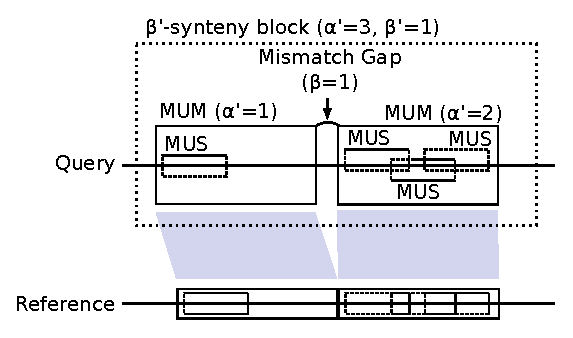
\includegraphics[width=1.0\columnwidth]{figures/02_contextschemes/MUMs.eps}
  \caption{Diagram of a $\beta^\prime$-synteny block for the $\alpha^\prime$-$\beta^\prime$-natural context scheme, composed of two MUMs.}
  \label{fig:model}
\end{figure}

\subsection{Credit}
%Introduce credit schemes

It is common to find some elements in a query string $x$ which are unmapped, and cannot be mapped on any extension of $x$, yet are intuitively recognizable as corresponding to reference positions. This often happens if bases are between two MUMs but are not part of any MUM themselves, or if they were part of a MUM between two other MUMs that cannot join a sufficiently $\alpha'$-separated $\beta'$-synteny block. In these cases, to create a scheme that maps more elements of the query,  we can augment our context assignments with additional contexts that allow such bases to map \vocab{on credit}, based on the mappings of the bases on either side. The particular credit method used here looks at the nearest mapped base on either side of a gap in mapping, and matches up elements with the correct bases with respect to their implied positions in the reference, allowing at most one mismatch. Previously unmapped elements that are matched to exactly one reference position will be mapped on credit, while elements that are matched to zero or two positions will not map.

Since only elements that did not already match, and which could not possibly match on any extension of the query, are mapped in this way, the addition of credit does not interfere with the nonredundancy of a context assignment or the stability of a context-driven mapping scheme.

% TODO: Make sure we are properly blacklisting bases from credit if they didn't map due to conflict, or are in MUMs too close to the ends.

\section{Results}
\label{sec:results}

%%Describe setup with the MHC

In order to test the utility of the theoretical constructs described here, a series of software tests were created in order to evaluate the mappings produced by the $\alpha$-$\beta$-natural scheme described above. Mapping accuracy was evaluated for both error-corrected long sequences and error-prone short sequences.

\subsection{Mapping MHC Alt Loci}

To evaluate the performance of the new mapping algorithms proposed here a long-sequence mapping task was defined. The human genome has, on chromosome 6, a region of approximately 5 megabases known as the \vocab{major histocompatibility complex (MHC)}, rich in antigen presentation genes vital to the function of the immune system \citep{the1999complete}.
The region is prone to complex rearrangement, is well-supplied with both coding and noncoding sequence, and exhibits extreme regional variation in the polymorphism rate along its span \citep{the1999complete}. As one of the most complex and difficult regions of the genome, it provides a good testbed for methods designed to deal with difficult structural variation. To better represent the complexity of this region, the Genome Reference Consortium (GRC)'s current human reference assembly (GRCh38) contains seven full-length MHC \vocab{alt loci}, each of which serves as a different alternate reference for the region \citep{church2011modernizing}. These alt loci come with official alignments to the chromosome 6 primary sequence, which are part of GRCh38 and were generated using the NGAligner tool and limited manual curation \citep{schneider2013genome,schneider2015grc}.

Each mapping scheme under test took the MHC alt loci (GI568335879, GI568335954, GI568335976, GI568335986, GI568335989, GI568335992, and GI568335994), and mapped each to the GRCh38 \vocab{primary path} region, which actually appears in the ``chr6'' FASTA record. The resulting alignments were compared against the official GRC alignments distributed with GRCh38, with the caveat that aligned, mismatched bases in the GRC alignments were de-aligned to ensure a fair comparison, as the mapping schemes being evaluated were not permitted to align mismatching bases together. (Allowing mismatching bases in the GRC alignments to align made no perceptible difference in any figure, and was not pursued further.) The standard information retrieval metrics of precision and recall against the GRC alignments were calculated using \texttt{mafComparator}, and can be seen in Figure~\ref{fig:mhcprecisionrecall} \citep{earl2014alignathon}. Overall coverage (the fraction of bases of an alt locus aligned to the reference), and the frequency and size of rearrangement events implied by the alignments, were also calculated, and are visible in Figure~\ref{fig:mhccoverage} and Figure~\ref{fig:rearrangements}, respectively.

%Coverage
%Min/max substring lengths
%Compare to ref. alignments, precision, recall
%Rearrangements
%Browser shots

\begin{figure*}[t]
  \centering
  \subfloat[]{
  	\label{fig:mhcprecisionrecall}
    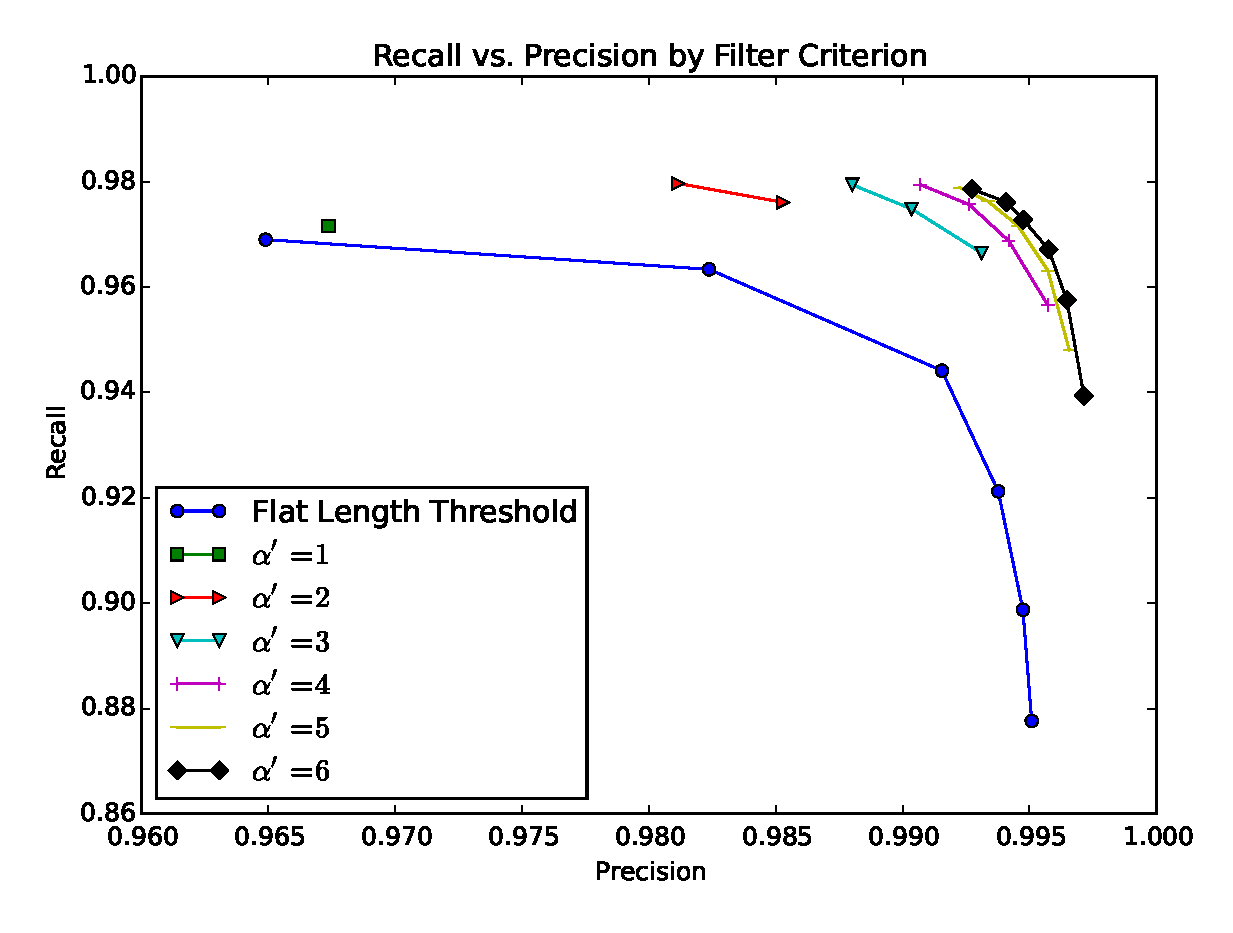
\includegraphics[width=0.5\textwidth]{figures/02_contextschemes/mhcPrecisionRecall.eps}
  }
  \subfloat[]{
  	\label{fig:mhccoverage}
    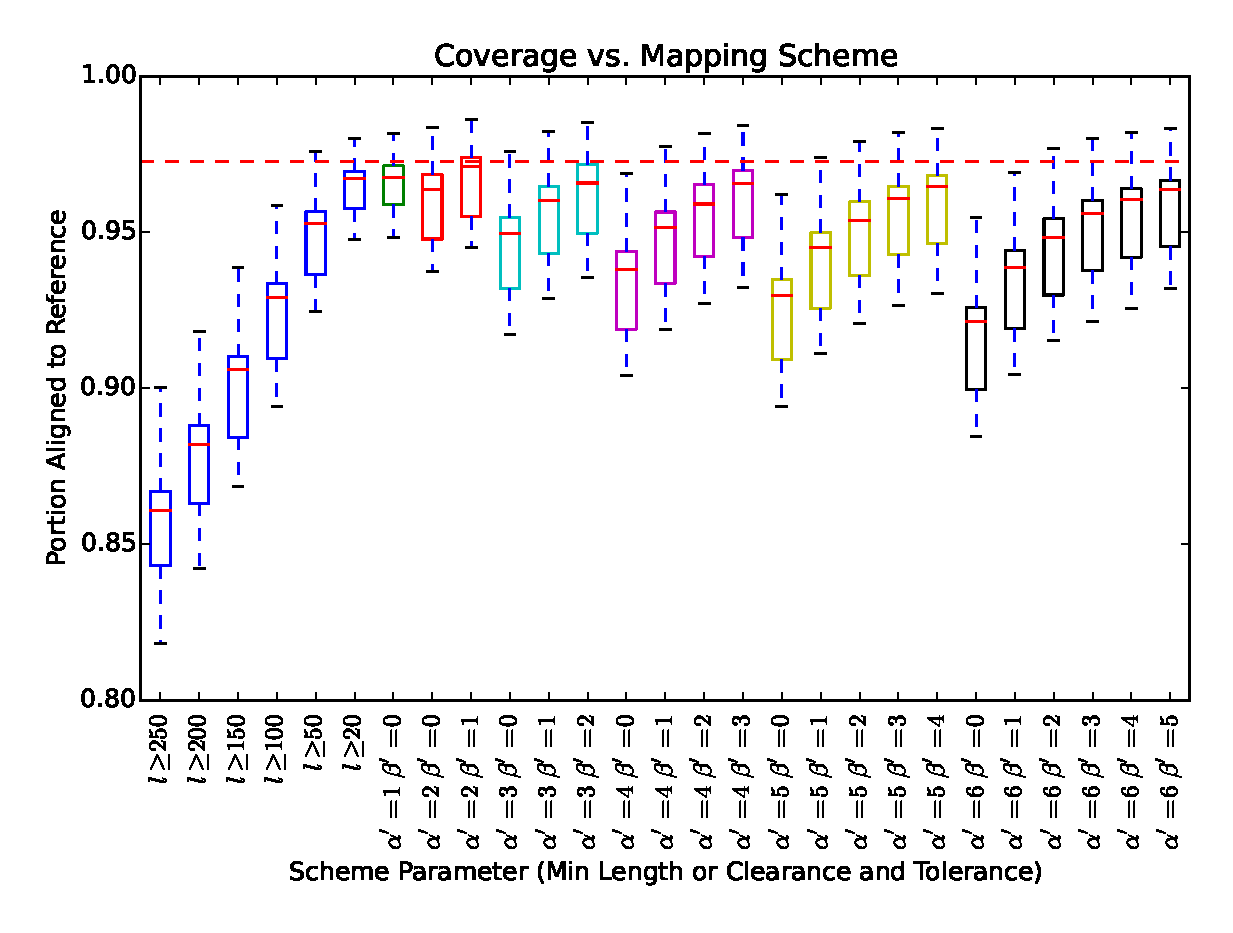
\includegraphics[width=0.5\textwidth]{figures/02_contextschemes/mhcCoverageBar.eps}
  }
  \caption{Results of MHC alignment. Points shown in \ref{fig:mhcprecisionrecall} are averages of alt-loci alignments. Lines connect different $\beta^\prime$ levels for a given $\alpha^\prime$. The red dashed line in \ref{fig:mhccoverage} is the average coverage of the GRC reference alignments.}
  \label{fig:mhc}
\end{figure*}


Mapping schemes using a wide range of $\alpha^\prime$ and $\beta^\prime$ parameters were tried, with $\beta'$ being restricted to values less than $\alpha'$. Additionally, the natural mapping scheme ($\alpha' = 0, \beta' = 0$) was tested, with a parameter used to vary the minimum length of admissible unique substrings (i.e. defining a series of natural context scheme, each only considering unique reference substrings longer than a minimum threshold). 

The strongest performing schemes, in terms of the harmonic mean of precision and recall (F-score), had a precision greater than 0.99 and a recall of around 0.98. Coverage was also remarkably close to that of the GRC reference alignments, suggesting that the conservative nature of the schemes did not result in undue underalignment (Figure~\ref{fig:mhccoverage}). 

In all cases the natural length-thresholded context schemes performed substantially worse than the various $\alpha^\prime$/$\beta^\prime$ combinations in terms of recall of the GRC alignments at a given level of precision (Figure~\ref{fig:mhcprecisionrecall}), and in terms of coverage (Figure~\ref{fig:mhccoverage}). This suggests that $\alpha^\prime$ and $\beta^\prime$ as defined here are effective heuristics. 

Increasing $\alpha'$ for a given $\beta'$ was found to increase precision and decrease recall, but increasing $\beta'$ at a given $\alpha'$ could restore the lost recall (at the cost of precision). The $\alpha' = 5, \beta' = 4$ natural scheme was determined to strike the best balance between precision and recall, as there was a negligible increase in precision between it and the $\alpha' = 6, \beta' = 5$ scheme (Figure~\ref{fig:mhcprecisionrecall}). Both it and the $\alpha' = 3, \beta' = 2$ scheme---selected to provide a good balance between precision and recall while also optimizing for mapping shorter sequences---were chosen for the short sequence mapping tests in \ref{subsec:reads} below.

Two additional configuration options were available for the schemes under test: whether to map unmapped internal bases on credit, and whether to enforce stability over weak stability. Our tests, the results of which are visible in Supplementary Figure~S1a and Supplementary Figure~S4b, demonstrate that requiring stability had a negligible impact on recall for long sequences, while the use of credit produced a sizable gain in recall at a manageable cost in precision (note the scales of the axes in Supplementary Figure~S4b). Consequently, credit was used for all analyses, and the stability requirement was used for the MHC mapping analysis.

\begin{figure}[t]
	\centering
    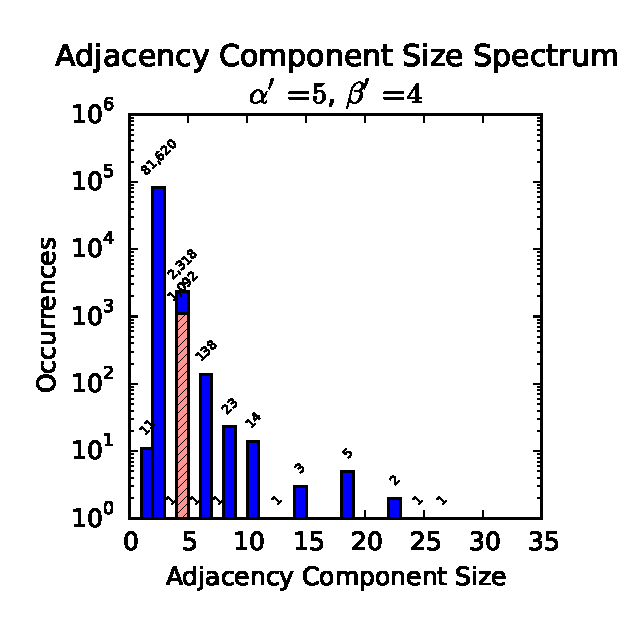
\includegraphics[width=0.3\textwidth]{figures/02_contextschemes/mhcRearrangements.eps}
  \caption{Frequency of rearrangements of different levels of complexity implied by the alignment of MHC alt loci to the primary path, under the $\alpha^\prime = 5$, $\beta^\prime = 4$ natural scheme, which was selected to give the best balance between precision and recall. The X axis shows the number of nodes involved in the rearrangement, while the Y axis shows the number of rearrangements of that size. The red bar shows the number of 4-node rearrangements that are automatically identifiable as tandem duplications.}
  \label{fig:rearrangements}
\end{figure}

%Revised to more precisely define the graph

The $\alpha^\prime = 5$, $\beta^\prime = 4$ natural scheme, which provided the best trade-off between precision and recall, was also evaluated in terms of the number and complexity of rearrangements it invoked to relate the MHC alt loci back to the primary path. Figure~\ref{fig:rearrangements} depicts a ``spectrum'' plot of rearrangement frequency versus size, where a rearrangement is defined as a connected component in a multi-breakpoint/adjacency %Cite needed - Medvedev multi-breakpoint graph/cactus graph theory paper
% BENEDICT TODO: Is this the one you meant?
graph representing the alignment between the primary reference sequence and an alt-loci sequence \citep{medvedev2007computability,paten2011cactus}. Briefly, the nodes of the graph are the ends (sides) of aligned sets of two or more bases and the edges the adjacencies, possibly containing interstitial unaligned sequence, that connect these ends \citep{medvedev2007computability,paten2011cactus}. The spectrum plot shows that the vast majority of rearrangements involve only two nodes (which is the structure of SNPs and simple indels), and of the rearrangements involving 4 nodes, slightly under half of them are recognizable as simple tandem duplications. The tandem duplications, which frequently involve just a handful of bases, are discoverable because of the non-linear nature of context-driven mapping. The remaining, more complex rearrangements have not been identified or named. Supplementary Figure~S5 shows UCSC Genome Browser renderings of some of the rearrangements described in the spectrum plot. 
% TODO: is there a reference to cite for this idea of pinch graphs? See above - Medvedev + cactus paper in JCB.
% See citations above. Would we maybe cite the pinchesAndCacti library?

\subsection{Mapping Simulated Short Reads}
\label{subsec:reads}

Perhaps the most important current application of traditional alignment methods is mapping reads from short read sequencing. To test this scenario a second mapping task was created. Each of the MHC alt loci sequences was broken into overlapping 200bp fragments at 100bp intervals. The read length was chosen to align with that of current or expected near future sequencing technologies, and is near the low end of what the mapping schemes presented here can accommodate \citep{quail2012tale}. Each of these fragments had substitution errors introduced with an independent probability of $1\%$ per base (comparable to current sequencing technologies) \citep{quail2012tale}. We used this simulated scenario, rather than actual reads, because it allowed us to assess the reads' origins to easily determine if mappings were correct or aberrant.


Two variants of the $\alpha'$-$\beta'$-natural scheme ($\alpha' = 3, \beta' = 2$, and $\alpha' = 5, \beta' = 4$), in both stable and weakly stable versions, were used to map each read to the primary path MHC from GRCh38. The results of the popular aligners BWA (using default parameters) and LASTZ (using an empirically-determined restrictive score cut-off), were also included \citep{li2010fast,harris2007improved}. BWA in particular functioned as a gold standard: we did not expect to outperform BWA, but rather sought to recapitulate some of its results in a context-driven framework.

Mapping accuracy was assessed in two ways. First, the number of reads that each mapper could place anywhere in the reference, and portion of bases mapped regardless of correctness, were measured. These results are visible in Figures~\ref{fig:readmappability} and~\ref{fig:readcoverage}, respectively. Second, the number of genes and portion of gene bases with incorrect mappings to other genes, as annotated by the UCSC Genome Browser's ``Known Genes'' database, were also measured, and are visible in Figures~\ref{fig:readgenes} and~\ref{fig:readwrongness} \citep{meyer2013ucsc}.  

%Paralogs
%Reads 
%-- error corrected reads
%-- non-error corrected reads

\begin{figure}[t]
  \centering
  \subfloat[]{
  	\label{fig:readmappability}
    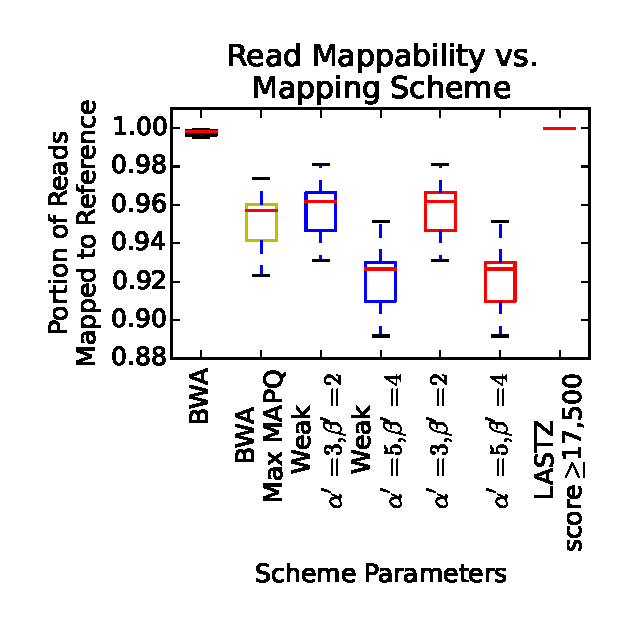
\includegraphics[width=0.5\columnwidth]{figures/02_contextschemes/readMappability.eps}
  }
  \subfloat[]{
  	\label{fig:readcoverage}
    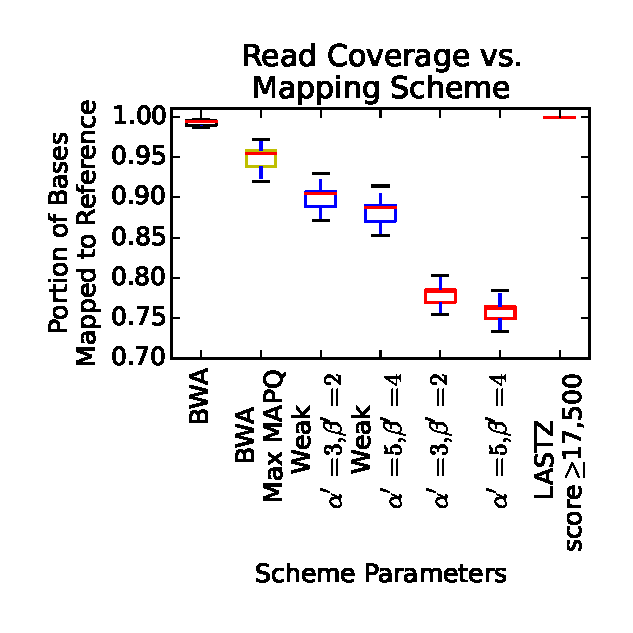
\includegraphics[width=0.5\columnwidth]{figures/02_contextschemes/readCoverage.eps}
  }
  \\
  \subfloat[]{
  	\label{fig:readgenes}
    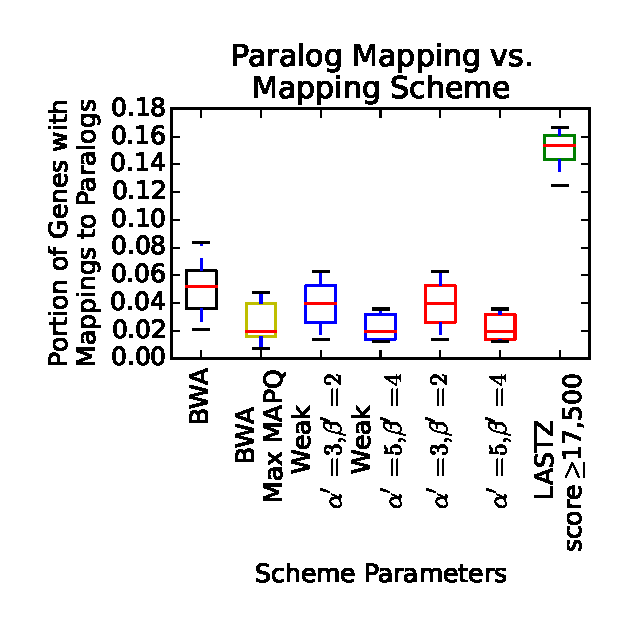
\includegraphics[width=0.5\columnwidth]{figures/02_contextschemes/readGenes.eps}
  }
  \subfloat[]{
  	\label{fig:readwrongness}
    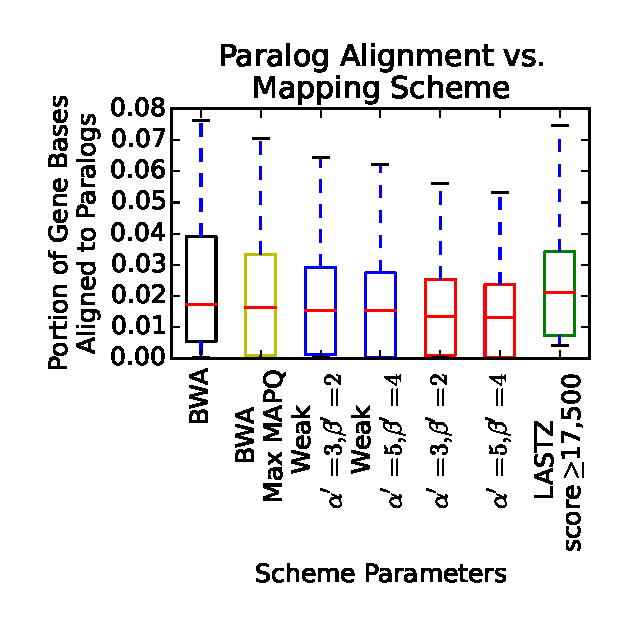
\includegraphics[width=0.5\columnwidth]{figures/02_contextschemes/readWrongness.eps}
  }
  \caption{Results of read alignments. Reads were generated from MHC alt loci by taking tiling 200bp windows at 100bp intervals, and randomly introducing substitution errors at a frequency of $1\%$. Reads were aligned to the GRCh38 primary path MHC region.}
  \label{fig:read}
\end{figure}

%It would be good to look at BWA positions that uniquely map (with no secondary alignments). 
BWA and LASTZ both mapped more of the reads and covered more of the read bases than the context-driven mapping schemes, though the difference was relatively small: less than 10\% in terms of mapped reads and, for the weakly stable context schemes, less than 15\% in terms of coverage. These results were unsurprising, given that a context-driven mapping scheme is a function that can not multi-map any position, while the other two aligners freely produced multi-mappings.

The context-driven mapping schemes examined broadly matched BWA's performance in terms of avoiding mapping genes to their paralogs (Figures~\ref{fig:readgenes} and \ref{fig:readwrongness}). All four context-driven schemes tested outperformed BWA's raw output. However, if BWA's output was filtered to only include reads mapped with maximum mapping quality (which was observed to be 60), only the $\alpha'=5$, $\beta'=4$ natural schemes managed to outperform it in terms of the portion of genes with any mappings to paralogs---and that at a very substantial drop in coverage (Figure~\ref{fig:readcoverage}). LASTZ, on the other hand, did not report mapping qualities; even with what was intended to be a stringent score threshold applied, it produced the most mappings to paralogs of any aligner tested (Figures~\ref{fig:readgenes} and \ref{fig:readwrongness}). 

While the difference between stable and weakly stable mapping schemes was insignificant for long-read mapping, the coverage difference for these shorter reads was much greater. Thus stability, rather than weak stability, might seem an impractical restriction for short reads, albeit one that still admits the mapping of the majority of query sequence elements.

A final experiment characterized the minimum context lengths with which it was possible for a base to map in the GRCh38 primary path MHC; the results are shown in Figure \ref{fig:contexts}. The vast majority of bases were found to be mappable with contexts of 100bp or less, and all but about $2\%$ of bases at $\alpha' = 5$ were found to be mappable with contexts of 200bp or less.


\begin{figure}[t]
  \centering
  \subfloat[]{
  	\label{fig:context}
    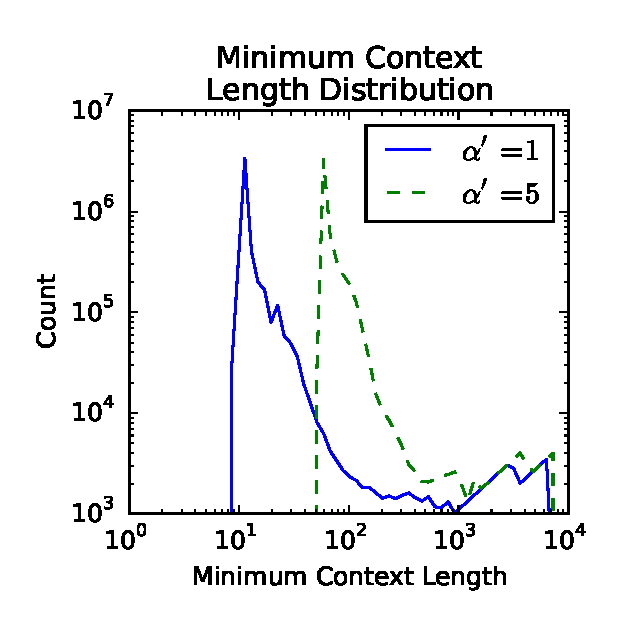
\includegraphics[width=0.5\columnwidth]{figures/02_contextschemes/context.eps}
  }
  \subfloat[]{
  	\label{fig:contextcumulative}
    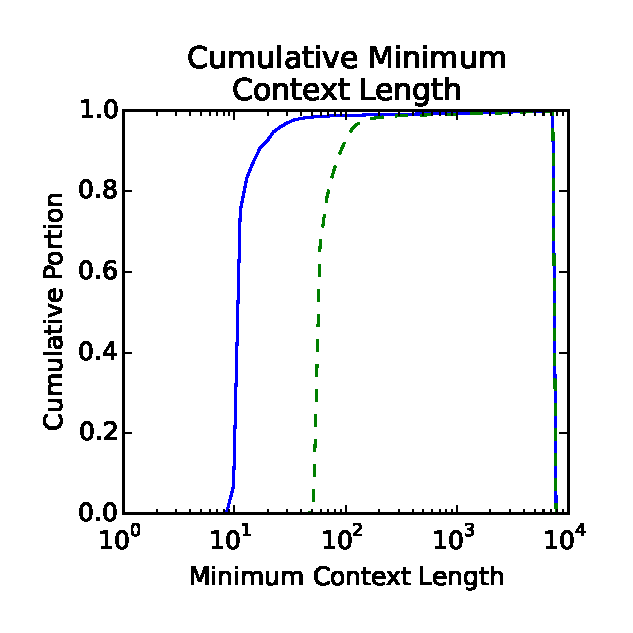
\includegraphics[width=0.5\columnwidth]{figures/02_contextschemes/contextcumulative.eps}
  }
  \caption{Minimum $\beta^\prime = 0$ context lengths required to map uniquely in a reference derived from the GRCh38 primary path MHC, for different $\alpha^\prime$ values. At an $\alpha^\prime$ of $1$, $1.16\%$ of minimal contexts are longer than 100bp, and $0.97\%$ are longer than 200bp. At an $\alpha^\prime$ of $5$, $8.85\%$ of minimal contexts are longer than 100bp, and $1.74\%$ are longer than 200bp}
  \label{fig:contexts}
\end{figure}

\section{Discussion}

%Give overview of benefits (basically the title of the paper)

The new mapping scheme proposed here---both radically different and more conservative than existing methods---has some important benefits. The first is that it is versatile: it can be used to map multi-megabase MHC sequences while accounting for complex rearrangements, but also does reasonably well with 200bp simulated reads. The second major benefit is stability: although requiring stability reduces coverage when mapping short reads, it reveals a majority subset of mapped positions that are aligned globally with high certainty. This is a useful per-base quality assessment somewhat orthogonal and complementary to the widely used read-level mapping quality scores \citep{li2008mapping}.
The third major benefit---being able to define variants in terms of canonical contexts which can diagnose their presence---is related to the second: having a stable mapping scheme enables the articulation of sequences which, when observed, always indicate the presence of a particular variant. This could ultimately pave the way for a high-specificity reference-free method of variant calling, building on the dbSNP concept of flanking strings \citep{sherry2001dbsnp}.

%Discuss how approach is conservative, but that is appropriate for certain cases


% Short sequence mapping

Our results show that the context-driven, stable mapping approach can be more conservative than existing mappers like BWA and LASTZ, at the cost of coverage. If there is any possibility of later having to admit that it was wrong in mapping a base, a stable scheme will not map that base. A weakly stable scheme is only slightly more permissive, willing to map bases only if it knows they cannot possibly map elsewhere. We show that the $\alpha'$-$\beta'$-natural schemes can be much more selective than LASTZ, and can in certain circumstances outperform BWA in avoiding mappings to paralogs, and in the general case are no worse. This specificity comes at the cost of a reduced ability to contend with high sequencing error rates. However, it is particularly important when analyzing regions like the MHC, where some genes present in a query may not be present themselves in the reference to which reads are being mapped, but may nonetheless have close and misleading paralogs in the reference. 
%Indeed, from this small study it is unclear how best to set $\beta'$ to ensure that paralogous mapping is minimized, and

%Cut for brevity
%As would be expected, the weakly stable mapping schemes appear to outperform the stable ones in terms of coverage, in Figure~\ref{fig:readmappability} and Figure~\ref{fig:readcoverage}. The short length of the sequences involved means that many poor MUMs which did not join a sufficiently good $\beta'$-synteny block are nonetheless heuristically regarded as potentially able to do so were the query sequence to be extended. If stability is required, bases which those MUMs cover are ``blacklisted'' and cannot be mapped anywhere. In order to reduce this performance gap, it will be necessary to compute a tighter bound on exactly which MUMs could potentially join a $\beta'$-synteny block with new MUMs that might be created when the query sequence is extended.

% Long sequence mapping
% Detected rearrangements

The $\alpha'$-$\beta'$-natural scheme presented here is more useful for mapping longer sequences, where the costs of stability (incurred only near the sequence ends) are lower, and the chances of finding longer and more distinctive contexts are higher. Longer reads are also more likely to directly exhibit some of the linearity-breaking structural rearrangements that our scheme is designed to deal with. The scheme presented here largely recapitulates the GRC's official alignments. The $\alpha' = 5, \beta' = 4$ instantiation, for example, has approximately $99\%$ precision and $98\%$ recall when compared to the GRC alignments, as depicted in Figure~\ref{fig:mhcprecisionrecall}. Given that the GRC alignments for the MHC alt loci do not contain any duplications, translocations, or inversions, some of the missing precision is almost certainly due to the correct detection of events that the GRC alignments did not completely describe. Judging by our manual analysis (illustrated in Supplementary Figure~S5), such calls are generally plausible. 

%Discuss extension to graphs.
Finally, the context-based mapping scheme method is abstracted from its reference and query inputs, and thus easy to generalize. In addition to being very general in the types of queries it can accept, from short reads to entire alt loci, it is also very general in the types of references it can map to. As long as context sets can be defined for each position, this method can be extended to map to nonlinear, graph-based reference structures (as in Supplementary Figure~S6). Such graph structures, containing common variation in addition to the primary reference, would help to alleviate the reference allele bias inherent in current approaches to variant detection. The mapping scheme presented here provides a concrete approach to mapping to such a structure, something we explored in our earlier paper \citep{paten2014mapping} and that we are actively pursuing. 

Future work to be done on this project includes the creation of a full alignment tool based on the algorithms described here, and an extension of those algorithms to graph-structured references. The software test framework created for this work is available from \url{https://registry.hub.docker.com/u/adamnovak/sequence-graphs/}.

\section*{Acknowledgements}

\paragraph{Funding}
This work was supported by a grant from the Simons Foundation (SFLIFE \#351901). AN was supported by research gift from Agilent Technologies, a fellowship from Edward Schulak, and an award from the ARCS Foundation. Research reported in this publication was also supported by the National Human Genome Research Institute of the National Institutes of Health under Award Number U54HG007990. The content is solely the responsibility of the authors and does not necessarily represent the official views of the National Institutes of Health.



\appendix
\chapter{Research Schedule}

\begin{table}[ht]
    \centering
    \begin{tabular}{l|c}
        \textbf{Task} & \textbf{Work Period} \\
        \hline
        Develop Mapping Scheme (\ref{subsec:aim1mapping}) & Q4 2014 \\
        Develop Merging Scheme (\ref{subsec:aim1merging}) & Q4 2014 \\
        Formalize Variant Mathematics (\ref{subsec:aim1math}) & Q1 2015 \\
        Scale to GRCh38 (\ref{subsec:aim2aligner}) & Q2 2015--Q4 2015 \\
        Add Additional Variation (\ref{subsec:aim2variation}) & Q1 2016 \\
        Build Reference Hierarchy APIs (\ref{subsec:aim2api}) & Q2 2016 \\
        Apply To NOTCH2NLs (\ref{subsec:aim3notch}) & Q3 2016 \\
        Re-Align Existing Data (\ref{subsec:aim3realign}) & Q4 2016 \\
        Maintain Reference Hierarchy (\ref{subsec:aim3maintenance}) & Q1 2017--Q2 2017 \\ 
    \end{tabular}    
    \caption{Research schedule for the proposed work.} 
    \label{tbl:schedule}
\end{table}


% %%%%%%%%%%%%%%%%%%%%%%%%%%%%%%%%%%%%%%%%%%%%%%%%%%%%%%%%%
% bibliography

% 2010june01 sol katzman:
% if \nocite is specified, all entries in the bib file are included,
% probably not what you want, so comment out the \nocite and only get the cited references.
%\nocite{*}

% 2010june01 sol katzman:
% this makes the bibliography single spaced, with double spacing between entries
\def\baselinestretch{1.0}\large\normalsize

% We need this for natbib for some reason
\def\newblock{\hskip .11em plus .33em minus .07em}
\bibliographystyle{plainnat}
\bibliography{thesis}

\end{document}
